\chapter{Realisation}
\section{Sensor data deserialistaion}
\section{Sensor data buffering}
\section{Data transfer}
\section{Synchronisation}
\section{Firmware}
\section{Tests}
%\subsection{ }
%\subsection{ }
%Potem pojawia się koncepcja w której opisujesz konkretna realizacje ze
%szczgolowym podzialem na bloki. Bez podawania schmatow ideowych.
%- układ deserializera
%- układ sekwencera
%- układ video DMA z buforami
%- układ generacji napiec i biasow
%- system Linuxowy i jego rola
%- interfejsy komunikacyjne. O SATA tylko wspominasz ze uruchomiles dla celów
%diagnostycznych.
%- oprogramowanie sterujace
%
%Jaki masz wkład naukowy?
%- opracowanie metody weryfikacji sprzętu bez dostępnego czujnika poprzez
%uzycie czujnika o podobnym interfejsie. Dzieki blokowej architekturze
%(frameworku) da się potem latwo podmienić czujnik.
%- opracowanie sposobu synchronizacji wielu kamer od strony sprzętowej i
%programowej
%- deserializacja sygnalu z interfejsow szeregowych czujnika ze sledzeniem
%fazy sygnalu. Przeciez w CMV to robiles.
%- weryfikacja oprogramowania i sprzętu metoda drobnych kroczków, czyli to co
%AGH na nas wymuszal. Testowanie wszystkich blokow a na samym końcu czujnika.
%
%Dalej przy testach oczywiście pokazujesz sygnal z czujnika CMV pisząc ze
%czujnik X nie był jeszcze gotowy do integracji bo w zasadzie nie był gdyż
%AGH nie pozwolil nam tego robic.
%Opisujesz metody testowania pamięci, Ethernetu, serializerow i
%deserializerow. Mase czasu nad tym spedziles. Podlaczenie czujnika to potem
%formalnosc


%
%\section{Introduction}
%This chapter presents the realisation of the master thesis. 
%This chapter is divided into five sections each describing the realisation of different part of the framework:
%\begin{itemize}
%    \item data transfer, precisely 1 Gigabit Ethernet and Serial ATA II
%    \item different operating system architectures, such as embedded Linux, Real-Time-Operating-System and Baremetal
%    \item video data acquisition from two types of sensors 
%    \item multi-camera synchronisation using Precision-Time-Protocol 
%    \item software based digital system control 
%\end{itemize}
%
%The work presented in this chapter provides new subsystems, which are a major improvement over existing vanilla
%components. Thus, allowing to resolve the main thesis problem - \textbf{the complexity of camera development.} 
%
%\section{Data transfer}
%Scientific camera design framework consists of two data transfer subsystems that were designed using partially existing
%components: 1 Gigabit Ethernet and Serial ATA II.   
%
%\subsection{1 Gigabit Ethernet}
%
%The implementation of 1 Gigabit Ethernet subsystem consists of:
%\begin{itemize}
%    \item digital system 
%    \item embedded Linux driver, scripts and socket server application
%    \item PC socket sever
%\end{itemize}
%
%Figure\ref{FIG:ETH} presents the block diagram of the 1000BASE-X subsystem design.    
%
%\begin{figure}[h!]
%    \centering
%    \includegraphics[width=13cm]{img/realisation/pcs_pma_ip_diag.png}
%    \caption{Block diagram of Camera framework Ethernet architecture}
%    \label{FIG:ETH}
%\end{figure}
%
%
%As stated in~[\ref{chapter4}] my work mostly consisted of the design of the digital system and the configuration 
%of embedded Linux . 
%
%The main technical difficulty of the implementation of 1 Gigabit Ethernet is the fact that the digital system has to
%be designed and tested together with firmware running on Cortex A9. Firmware working on multiple levels is needed to
%make the subsystem work, precisely:
%\begin{itemize}
%    \item Linux Kernel driver 
%    \item FSBL (first stage bootloader)
%    \item device tree
%    \item Linux script to load the driver
%    \item Linux application (websocket server)
%\end{itemize}
%
%\subsubsection{Digital system design}
%The digital system side of the 1 Gigabit Ethernet consists of:
%\begin{itemize}
%    \item Xilinx 1000BASE-X PCS/PMA IP Core - Functions as a PHY device between the SGMII interface on the MAC and the SFP transceiver on the board. 
%    \item Zynq Processing System - Master of the interface, with built in MAC. 
%    \item Constant value IP - Static IP for setting correct values on the IP Core
%\end{itemize}
%
%Two methodologies were used in the design of the 1000BASE-X interface for camera framework, due to the fact
%that block design is necessary for the use of Zynq SoC and because several functions had to be done in the pure
%VHDL. 
%
%\paragraph{Subsystem requirements}\mbox{}\\
%The requirements for 1 GbE Ethernet subsystem is a sum of requirements of specific components, mainly:
%\begin{itemize}
%    \item 125 MHz external low noise clock signal needs to be connected to the GTX clock input of the SoC  
%    \item 100 MHz internal clock signal connected using BUFG\ref{XIL:TRM}  
%    \item GTX data lines needs to be connected to a SFP cage, where a transceiver can be placed
%    \item Zynq Processing System needs to use one of it's GPIOs to control the IP Core
%\end{itemize}
%
%\paragraph{Design process}\mbox{}\\
%The following steps were done in order to implement the digital system for the 1000Base-X:
%\begin{enumerate}
%    \item block design was added to the project
%    \item Zynq Processing System was added to the block design with the following configuration:
%        \begin{itemize}
%            \item FCLK0 enabled set to 100 MHz - for the internal clock
%            \item GPIO enabled ( 1 bit ) exported externally so that it can access digital system
%            \item Ethernet MAC exported to the digital system (EMIO) so that SGMII interface can be used
%            \item clock signal to the MAC was set to an external one and the data throughput is set statically to 1 Gbps
%        \end{itemize}
%
%    \item 1 GbE PCS/PMA IP Core was added to the design block with following configuration:
%        \begin{itemize}
%            \item Ethernet MAC - set to Zynq PS Gigabit Ethernet Controller
%            \item Standard - 1000BASEX, additional transceiver control and status ports not enabled 
%            \item Core Functionality - Device Specific Transceiver, MDIO for external PHY not enabled, PHY Address: 6 
%            \item Shared Logic - turned on 
%        \end{itemize}
%
%
%    \item constant value set of registers was connected to the inputs of the 1 GbE PCS/PMA IP Core to fix the values
%        of the input configuration signals and registers
%    \item SGMII from Zynq's MAC was connected to the 1 GbE PCS/PMA IP Core 
%    \item 100 MHz FCLK0 clock was connected to the input internal clock of the PCS/PMA IP Core
%    \item the 1 GbE PCS/PMA IP Core SFP differential pairs were exported to as a port from block design
%    \item the wrapper from block design was generated and instantiated to the top entity
%    \item the constraints were added to the project for the correct pinout and clock signals parameters 
%    \item the design was successfully synthesised and implemented, no simulations were performed, due to the fact
%        that they are very limited with Zynq Processing System
%\end{enumerate}
%
%Figures \ref{FIG:PCS_PMA_CONFIG},\ref{FIG:PCS_PMA_CONFIG2} present the configuration window of the PCS/PMA IP Core in Vivado
%and connections between the Zynq and the PCS/PMA IP Core.    
%
%\begin{figure}[H]
%    \centering
%    \includegraphics[width=13cm]{img/realisation/pcs_pma_config.PNG}
%    \caption{Configuration of Ethernet 1000BASE-X PCS/PMA IP Core}
%    \label{FIG:PCS_PMA_CONFIG}
%\end{figure}
%
%\begin{figure}[H]
%    \centering
%    \includegraphics[width=13cm]{img/realisation/pcs_pma_zynq_config3.PNG}
%    \caption{Connection between Zynq Processing System and Ethernet 1000BASE-X PCS/PMA IP Core}
%    \label{FIG:PCS_PMA_CONFIG2}
%\end{figure}
%
%\subsubsection{Embedded Linux}
%The general configuration of embedded Linux for the camera framework is presented in the next section. Specific
%configuration regarding the use of Ethernet 1000BASE-X interface is presented here.
%
%In order to provide support for the 1000BASE-X the following parts of the operating system had to be modified:
%\begin{itemize}
%
%    \item Configuration
%    \item Kernel patching
%    \item Device Tree
%    \item System applications
%
%\end{itemize}
%
%\paragraph{Configuration}
%The main aspects of Petalinux configuration for Ethernet subsystem was enabling the following options in the Kernel
%configuration:
%\begin{lstlisting}
%    CONFIG_NET_VENDOR_XILINX=y
%    CONFIG_XILINX_EMACLITE=y
%    CONFIG_XILINX_AXI_EMAC=m
%    CONFIG_XILINX_PS_EMAC_EMIO=m
%    CONFIG_XILINX_PS_EMAC=y
%\end{lstlisting}
%
%This options set the EMACPS\_EMIO driver as a module so it can be loaded at any time. It is not recommended to set it to
%load automatically, because the clock signal to the GTX transceivers has to be present and of right frequency (125 MHz)
%in order to properly initialise the PCS/PMA IP Core. 
%    
%\paragraph{Kernel patching}\mbox{}\\
%Xilinx provides a Kernel patch to add support for the PCS/PMA IP Core. Kernel patch needs to be applied after
%configuration of Petalinux. It adds the Si5234 clock signal generator driver and PCS/PMA driver.   
%
%The patch has to be applied before the compilation of the kernel sources. 
%
%\paragraph{Device Tree}\mbox{}\\
%
%\emph{A device tree is a data structure describing hardware}~\cite{WWW:LINARO}. Embedded Linux uses a Device Tree Blob 
%as a reference for the peripherals. It contains information regarding the physical address and the driver name for
%specific devices~\cite{LNX:DEVICE_TREE}~\cite{XIL:DEVICE_TREE}. The introduction of a Device Tree Blob has made the
%creation of operating systems more 
%flexible, especially for embedded systems using SoCs where the configuration of
%the Main Processing Unit may differ greatly from one device to another. 
%
%Listings~\ref{LST:DEVICE_TREE}\ref{LST:DEVICE_TREE2} present the added portion of the device tree apart from the one created automatically by
%the \textbf{petalinux-build} program. Figure~\ref{fig:device_tree_structure} presents the Device Tree structure that is
%used in the Camera System. 
%
%\begin{figure}[h!]
%    \centering
%    \includegraphics[width=10cm]{img/realisation/device_tree_diag.png}
%    \caption{Device Tree structure of a camera system}
%    \label{fig:device_tree_structure}
%\end{figure}
%
%The main Device Tree file includes the dedicated configuration of the SoC: the address space of dynamic memory,
%configuration of Ethernet MAC (gem1), UART and I2C protocol devices listing. The embedded Device Tree configuration file
%contains more specific configuration - what is connected to AMBA/AHB bus in Programmable Logic. The configuration of 
%an embedded register in Programmable Logic sets the address where the register is placed in the physical address space 
%and also that the UIO (User Space Input/Output) driver is going to be used for its control. 
%
%The use of UIO greatly simplifies the use of any custom IP Core embedded in Programmable Logic due to the fact that
%there is no need for developing your own driver. UIO drivers allow for direct write and read to specific address memory
%space which, in the case of an embedded register for example, will set the value of a specific register.  
%
%A device tree is loaded during the system boot by bootloader along with the kernel.  
%
%\begin{lstlisting}[language=xml,caption=Device tree camera.dtsi file, label=LST:DEVICE_TREE]
%{
%    amba_pl: amba_pl {
%        #address-cells = <1>;
%        #size-cells = <1>;
%        compatible = "simple-bus";
%        ranges ;
%
%        IO_axi_quad_spi_0: axi_quad_spi@41e00000 {
%            compatible = "xlnx,xps-spi-2.00.a","xlnx,xps-spi-2.00.a";
%            interrupt-parent = <&intc>;
%            interrupts = <0 29 1>;
%            status = "okay";
%            reg = <0x41e00000 0x10000>;
%            num-cs = <0x5>;
%        };
%
% ctrl_reg: ctrl_reg3@43c00000 {
%        compatible = "generic-uio";
%        reg = <0x43c00000 0x10000>;
%        xlnx,s00-axi-addr-width = <0x6>;
%        xlnx,s00-axi-data-width = <0x20>;
%    };
%};
%};
%\end{lstlisting}
%
%\begin{lstlisting}[language=xml,caption=Device tree system.dtsi file, label=LST:DEVICE_TREE2]
%/dts-v1/;
%/include/ "zynq-7000.dtsi"
%/include/ "camera.dtsi"
%
%/ {
%    model = "Camera v1.0";
%    compatible = "xlnx,zynq-7000";
%
%    aliases {
%        ethernet0 = &gem1;
%        i2c0 = &i2c0;
%        serial0 = &uart1;
%        spi0 = &qspi;
%    };
%
%    memory {
%        device_type = "memory";
%        reg = <0x0 0x40000000>;
%    };
%
%    chosen {
%        bootargs = "console=ttyPS0,115200 root=/dev/ram rw earlyprintk";
%        linux,stdout-path = "/amba/serial@e0001000";
%    };
%};
%
%&gem1 {
%    compatible = "xlnx,ps7-ethernet-emio-1.00.a";
%    status = "okay";
%    phy-mode = "rgmii-id";
%    phy-handle = <&phy1>;
%    gt-reset-gpios = <&gpio0 54 1 >;
%
%    phy1: phy@6 {
%        reg = <6>;
%    };
%};
%
%&i2c0 {
%    status = "okay";
%    clock-frequency = <400000>;
%
%        i2c@0 {
%            #address-cells = <1>;
%            #size-cells = <0>;
%            reg = <2>;
%            eeprom@54 {
%                compatible = "at,24c08";
%                reg = <0x54>;
%            };
%        };
%
%        i2c@1 {
%            #address-cells = <1>;
%            #size-cells = <0>;
%            reg = <0>;
%            si570: clock-generator@5d {
%                #clock-cells = <0>;
%                compatible = "silabs,si570";
%                temperature-stability = <50>;
%                reg = <0x5d>;
%                factory-fout = <200000000>;
%                clock-frequency = <100000000>;
%            };
%        };
%
%        i2c@2 {
%            #address-cells = <1>;
%            #size-cells = <0>;
%            reg = <0>;
%            fan_ctrl@5e {
%                compatible = "mi,max6639";
%                reg = <0x5e>;
%            };
%        };
%};
%
%&sdhci0 {
%    status = "okay";
%};
%
%&uart1 {
%    status = "okay";
%}
%\end{lstlisting}
%
%
%\paragraph{System applications}\mbox{}\\
%The main system application regarding the 1000BASE-X support were: websocket server and initialisation scripts. 
%Websocket server was written by BSc. Damian Krystkiewicz and MEng. Maciej Trochimiuk. The scripts
%provided the functionality of: reconfiguring the Si570 clock signal generator, loading and initialising the PCS/PMA IP
%Core. In order to load the driver the \textbf{root} user has to log in to the operating system, this is performed by
%\textbf{autologin} application, and the loading itself is done by another script which modifies the \textbf{.profile}
%script of the root user and configures the network.   
%
%
%The way the application can be added to Petalinux is through the use of \textbf{petalinux-create} command.
%This creates a draft of an application and adds it to the boot sequence of the OS. This system has some limitations,
%such as, there is no way to control the order of the execution of the applications during boot (it can be done
%manually). Nevertheless the script for the \textbf{autologin} application has been created and modified so that it works
%correctly with the program.  
%
%\begin{lstlisting}[caption=Autologin initialistaion script, language=bash]
%ifndef PETALINUX
%$(error "Error: PETALINUX environment variable not set. 
%Change to the root of your PetaLinux install, and source the settings.sh file")
%endif
%
%include apps.common.mk
%
%APP = autologin
%
%# Add any other object files to this list below
%APP_OBJS = autologin.o
%
%all: build install
%
%build: $(APP)
%
%$(APP): $(APP_OBJS)
%$(CC) $(LDFLAGS) -o $@ $(APP_OBJS) $(LDLIBS)
%
%clean:
%-rm -f $(APP) *.elf *.gdb *.o
%
%.PHONY: install image
%
%install: $(APP)
%#	$(TARGETINST) -d $(APP) /bin/$(APP)
%$(TARGETINST) -d -p 0755 autologin /etc/init.d/autologin
%$(TARGETINST) -s /etc/init.d/autologin /etc/rc5.d/S99autologin
%
%          %.o: %.c
%$(CC) -c $(CFLAGS) -o $@ $<
%
%help:
%@echo ""
%@echo "Quick reference for various supported build targets for $(INSTANCE)."
%@echo "----------------------------------------------------"
%@echo "  clean              clean out build objects"
%@echo "  all                build $(INSTANCE) and install to rootfs host copy"
%@echo "  build              build subsystem"
%@echo "  install            install built objects to rootfs host copy"
%
%\end{lstlisting}
%
%\begin{lstlisting}[caption=Autologin application, language=C]
%
%/*
%*
%* Autologin application. 
%* Ethernet doesn't want to start when there is no user logged in.
%*
%*/
%#include <unistd.h>
%#include <stdio.h>
%
%int main(int argc, char *argv[])
%{
%
%  execlp("login","login","-f","root",0);
%
%}
%
%
%\end{lstlisting}
%
%
%\begin{lstlisting}[caption=PCS/PMA IP Core driver loading script, language=bash]
%#!/bin/sh
%
%# Startup script for setting ethernet using a kernel module for PCS/PMA
%# Author: Piotr Zdunek
%# Date: 04.01.2016
%
%echo "Setting up Ethernet.."
%echo "Loading Ethernet kernel module..."
%EMACPS_DIR=`find /lib -name xilinx_emacps_emio.ko`
%
%insmod $EMACPS_DIR
%
%# do not setup ethernet before kernel module is properly loaded
%wait
%
%echo "Setting up profile.."
%touch /home/root/.profile
%echo "echo CAMERA v1.0" >> /home/root/.profile
%echo "ifconfig eth0  up" >> /home/root/.profile
%
%camera-server --ControllerPort=500 --DataPort=700 \ 
%--MaintenancePort=600 --LogFile=log.txt &
%
%\end{lstlisting}
%
%
%\subsubsection{Ethernet tests}
%Basic ethernet tests were perfomed when the subsystem was ready, mainly:
%\begin{itemize}
%    \item \textbf{ifconfig} ethernet setup on petalinux
%    \item \textbf{ping} test to a remote PC
%    \item \textbf{iperf} tests to measure performance
%\end{itemize}
%
%More thorough tests were performed by Xilinx\cite{XIL:ETH_TESTS}, figure\ref{FIG:ETH_PERF} presents throughput test
%of the 1 GbE done in a similar way in programmable logic by Xilinx. 
%
%\begin{figure}[h!]
%    \centering
%    \includegraphics[width=10cm]{img/realisation/eth_perf_xil.png}
%    \caption{Performance tests of Ethernet done by Xilinx\cite{XIL:ETH_TESTS}}
%    \label{FIG:ETH_PERF}
%\end{figure}
%
%
%
%\subsection{Serial ATA II}
%
%The implementation of the subsystem of Serial ATA II was done entirely in programmable logic. The reason for this was to make it
%easy to transfer the data from the camera sensor to the hard drive. Serial ATA II IP Core was obtained from \url{opencores.org} 
%which is an open-source community 
%providing IP Cores for FPGAs. 
%
%The IP Core implements the \textit{Command}, \textit{Transport} and \textit{Link} layers of Serial ATA interface. It
%also provides a means for communicating IP with the physical layer GTX Transceivers. The physical layer module contains
%a finite state machine to drive the Out-Of-Band signalling used for initialization and synchronisation of SATA interface.
%The IP allows for transferring data with Hard Drives compatible with SATA 2 (Winchester) and with SSD Flash drives. 
%
%The main technical challenge was to make it work on 7 Series FPGAs and to provide the
%possibility to write to multiple hard drives simultaneously. The  SATA IP was targeted for Virtex 6 devices, 
%and thus it had to be redesigned to support the 7 Series Xilinx FPGAs.  
%
%%
%Virtex 6 devices allow for synthesising a clock signal for high-speed transceivers internally. This is a major difference
%between the Series 7 Xilinx FPGAs and series 6. Mgr inż. Adrian Byszuk was responsible for making the IP core running on
%Kintex 7 device. This was done by modifying the internal structure of the IP so that it conforms to the clocking
%architecture of the GTX transceivers in Xilinx FPGA.   
%
%\paragraph{IP Core signals}\mbox{}\\
%\begin{lstlisting}[caption=SATA IP Core signals, language=XML]
%
%PORTS: 
%            -- Command, Control and Status --
%
%ready_for_cmd          :  When asserted, SATA core is ready to execute 
%                          new command. This signal goes low after new_cmd 
%                          is asserted. It also serves as the command done signal    
%new_cmd                :  Asserted for one clock cycle to start a request        
%cmd_type               :  "01" for READ request and "10" for WRITE request	          
%sector_count           :  Number of sectors requested by user 
%sector_addr            :  Starting address of request
%
%            -- Data and User Clock --
%
%sata_din               :  Data from user to Write to Disk  
%sata_din_we            :  Write Enable to SATA Core when FULL is low 
%sata_core_full         :  SATA Core Full- de-assert WE 
%sata_dout              :  Data output from SATA Core
%sata_dout_re           :  Read Enable from SATA asserted when EMPTY is low 
%sata_core_empty        :  SATA Core Empty- de-assert RE
%SATA_USER_DATA_CLK_IN  :  SATA Core Write Clock  
%SATA_USER_DATA_CLK_OUT :  SATA Core Read Clock
%sata_timer             :  SATA core timer output to check performance 
%
%             --PHY Signals--
%CLKIN_150              :  150 Mhz input reference clock for the GTX 
%                          transceivers
%reset                  :  Resets GTX and SATA core; can be tied to 
%                          a software reset
%
%LINKUP                 :  Indicates Link Initialization done (OOB) 
%                          and SATA link is up 
%
%--GTX transmit/receive pins
%TXP0_OUT, TXN0_OUT, RXP0_IN, RXN0_IN                		
%\end{lstlisting}
%
%The IP Core itself consists of several files: 
%
%\begin{itemize}
%\item \textit{command\_layer.vhd} command layer interface
%\item \textit{crc.vhd} crc calculation
%\item \textit{ipcores.v} transceivers IPs
%\item \textit{mux\_21.v} multiplexer 2bit 2:1.
%\item \textit{mux\_41.v} multiplexer 32bit 4:1.
%\item \textit{mux\_161.v} multiplexer 32bit 16:1.
%\item \textit{oob\_control.v} out-of-band (oob) initialisation and synchronisation
%\item \textit{sata\_core.v} top file 
%\item \textit{sata\_link\_layer.v} SATA link layer 
%\item \textit{scrambler.v} SATA scrambler
%\end{itemize}
%
%Initial tests performed on the IP Core were successful and allowed for read and write data to an SSD. 
%Tests were done using data from the sensor. The amount of data coming from the CMV4000
%sensor was higher than the bandwidth of a single hard drive, for this reason multiple hard drive configuration was
%created. The table \ref{TBL:SSD_SENSOR} presents the difference in the throughput between the sensor and single hard
%drive. 
%
%
%        \begin{table}
%            \centering
%            \caption{Throughput comparison between single SSD and CMOS sensor}
%            %\begin{tabular}{|p{3cm}||p{5cm}|p{5cm}|}
%            \begin{tabularx}{\textwidth}{|l|X|X|}
%                \hline
%                & \textbf{Single SSD}  & \textbf{CMOS Sensor(CMV4000)}  \\ 
%                \hline
%                \hline
%                \textbf{Data}    & 
%                \vspace{0.1cm}
%                150 MHz x 32 bit = 515 MB/s
%                & 
%                \vspace{0.1cm}
%                40 MHz x 16 ch x 12 bit = 916 MB/s\\  
%                \hline
%            \end{tabularx}
%            \label{TBL:SSD_SENSOR}
%        \end{table}
%
%
%This shows that at least two SSDs have to be used to \emph{directly} store data coming from the sensor to the SSDs. 
%
%\paragraph{Dual hard drive configuration}\mbox{}\\
%Unfortunately, the modified clocking architecture for the IP Core did not support the use of multiple IP Cores in the
%same clock domain, which is necessary for the raw data acquisition from the CMV4000 sensor. 
%
%In order to use multiple IP Cores with the same single clock signal, some modifications were made:
%\begin{itemize}
%    \item re-routing the IBUFGDS differential clock buffer from within the core, outside to the wrapper
%    \item for the multiple IPs in the same domain scenario, QPLL based clocking distribution had to be implemented 
%\end{itemize}
%
%The first change was necessary for the multiple IP configuration to work. IBUFGDS is a Xilinx Series 7 FPGA
%primitives~\cite{XIL:PRIMITIVES} which is a differential input buffer for high speed clock signals used in GTX
%transceivers. Originally, the IP Core was designed so that the differential clock signal entering the device was routed
%internally to the IP Core, where it was changed to a single-ended signal using IBUFGDS. Unfortunately, this limits
%the use of the Serial ATA IP to a single instance for a Quad to which a 150 MHz differential clock signal is connected.  
%This is an unrealistic constraint for any design, since it is unknown how much storage is going to be required in
%camera designs. For this reason, the IBUFGDS was rerouted to the outside buffer so that the global entity of the Serial
%ATA IP Core was using a single-ended clock for the transceivers. This way one can attach a single 150 MHz clock signal to
%the quad and run up to 4 SATA links synchronously. 
%
%Xilinx GTX Quad contains 4 channels. Figure~\ref{FIG:GTX_QUAD} presents the architecture of the Xilinx GTX transceiver Quad. 
%
%\begin{figure}[h!]
%    \centering
%    \includegraphics[width=9cm]{img/realisation/gtx.png}
%    \caption{Block diagram of Xilinx 7 Series GTX Quad\cite{XIL:GTX}}
%    \label{FIG:GTX_QUAD}
%\end{figure}
%
%In order to achieve a synchronous design between multiple channels within the Quad using a single clock, a common clock
%has to be used and routed using QPLL. It is important to note, that one
%instantiation of the SATA IP Core has to have QPLL generic option enabled, whereas the rest, connected to the same quad,
%have to have QPLL generic option \textbf{disabled}. This is due to the fact that there is only one QPLL per quad, so it is
%impossible to instantiate multiple QPLLs. Furthermore, the maximum number of high speed channels in one quad is four. 
%For more channels, one has to use multiple quads and connect a separate clock signal to each quad. 
% 
%
%%Figure~\ref{FIG:SATA_FSM} presents the way thte state machine work for SATA.  
%%
%%%
%\paragraph{Control state machine}
%In the main wrapper of the camera framework a Finite State Machine was designed in order to transfer the data using
%SATA interface. The start of the sensor data acquisition and saving of the data on the hard drive are set using the
%configuration register through AXI bus using Zynq processor.   
%
%
%
%%%\begin{tikzpicture}[->,>=stealth',shorten >=1pt,auto,node distance=2.8cm,
%%%    semithick,minimum size=35pt]
%%%    \tikzstyle{every state}=[fill=white,draw=black,text=black,minimum size=35pt]
%%%
%%%    \node[state] (A)                    {reset};
%%%    \node[state]         (B) [below of=A] {wait for\\ linkup};
%%%    \node[state]         (D) [below of=B] {state1};
%%%    \node[state]         (C) [below of=D] {state2};
%%%    \node[state]         (E) [below of=C] {state3};
%%%
%%%    \path (A) edge [loop above] node {rst = 1} (B)
%%%          (B) edge node {linkup = 1} (D)
%%%          %(B) edge [loop above] node {1,1,L} (B)
%%%          (D) edge node {test} (C)
%%%          (C) edge node {0,1,L} (E);
%%%%        edge [bend left]  node
%%%%        {1,0,R} (E)
%%%%        (D) edge [loop
%%%%        below]
%%%%        node
%%%%        {1,1,R}
%%%%        (D)
%%%%        edge
%%%%        node
%%%%        {0,1,R}
%%%%        (A)
%%%%        (E)
%%%%        edge
%%%%        [bend
%%%%        left]
%%%%        node
%%%%        {1,0,R}
%%%%        (A);
%%%    \end{tikzpicture}
%%%
%
%
%\subsubsection{Functional specification}
%
%\subsubsection{Subsystem requirements}
%
%\subsubsection{Implementation}
%
%\subsubsection{Tests}
%
%\section{Operating system architecture}
%\subsection{Embedded Linux}
%
%
%The embedded operating system running on the camera is a Xilinx distribution of Linux: Petalinux \cite{XIL:PETALINUX}.
%The Petalinux system provides an easy way to configure and setup an operating system for Zynq SoC and also for Microblaze. 
%The configuration is done using a set of tools provided by the vendor. On the one hand, Petalinux makes it possible to
%quickly design a system, but on the other it makes it less versatile and flexible. 
%
%What is essential is that Petalinux kernel provides a set of drivers and programs dedicated specifically for Zynq SoC. 
%These drivers make it possible to easily use IP Cores added to Programmable Logic from Linux OS. Additionally, an
%automatic \textit{Device-Tree} generation is also performed, which takes into account the added IP Cores to the digital
%system.  
%
%Petalinux generates the following files which are then used as a system image: 
%\begin{itemize}
%    \item \textbf{FSBL} - first stage bootloader - which is a baremetal ARM A9 application which sets all the necessary
%        configurations such as boot source during runtime 
%    \item \textbf{uboot} - a Linux bootloader
%    \item \textbf{image.ub} - system image 
%    \item \textbf{bitstream.bit} - a bitstream file for FPGA configuration
%\end{itemize}
%
%The FSBL and \textit{ps\_init} files are automatically generated with the petalinux project. It is worth noting that configuration of
%peripherals before Linux boot can be performed only if the booting of the system is being done either using SD Card or
%Flash memory. It cannot be performed by booting the system through JTAG due to a different order of loading system image
%and bitstream. 
%
%Another key aspect of Petalinux is that it is based on \textit{yocto}~\cite{WWW:YOCTO}, which is an alternative to
%\textit{buildroot} embedded Linux system design platform. This makes it easier to adjust and modify based on yocto
%documentation.   
%
%\subsubsection{Configuration}
%
%First of all, IP core configuration in Block Design is exported to HDF\footnote{Hardware Description File}. 
%This file is put into the Petalinux project in order for the tools to create the configuration for the OS based on 
%what has been designed in Programmable Logic. This is done using  \textbf{petalinux-config} 
%program with option \textbf{--get\_hw\_description} flag. An example of the full command is listed below.  
%
%\begin{lstlisting}
%pzdunek$zdunek:~$ petalinux-config --get-hw-description=. 
%\end{lstlisting}
%
%%\subsubsection{Main configuration}
%
%The next step of creating the Petalinux OS is the configuration of specific parts of the system:kernel, bootloader
%and rootfs. The main configuration of Petalinux is done using the \textbf{petalinux-config} command. 
%%
%%\begin{figure}[H]
%%    \centering
%%    \includegraphics[width=13cm]{img/realisation/petalinux_config.png}
%%    \caption{Configuration window of petalinux-config program}
%%    \label{fig:petalinux_config}
%%\end{figure}
%
%
%This configuration program allows for choosing a specific kernel, bootloader, rootfs and also the place in address
%space of each component. For this camera project, a specific version of kernel was used in order for PCS/PMA IP Core
%to work. This setting is done in accordance to Xilinx Application Note~\cite{XIL:ZYNQ_PL_ETH}.
%Figure~\ref{fig:petalinux_config_kernel_1} presents an example of configuration setup screen. 
%
%\begin{figure}[h!]
%    \centering
%    \includegraphics[width=13cm]{img/realisation/petalinux_config2.png}
%    \caption{Configuration of Kernel source}
%    \label{fig:petalinux_config_kernel_1}
%\end{figure}
%
%
%\paragraph{Kernel}\mbox{}\\
%
%In order to configure the Kernel, the designer has to use \textbf{petalinux-config} program with option \textbf{ -c
%kernel}. The following options were selected in the kernel configuration: 
%
%\begin{itemize}
%    \item kernel set to remote (for PCS/PMA IP Core)
%    \item early kernel error messages on (EARLYPRINTK=y)
%    \item added support for REMOTEPROC and RPMSG for multicore communication
%    \item UART1 is set as standard output
%\end{itemize}
%
%%    Figure~\ref{fig:petalinux_kernel_config} presents the main windows of the configuration. 
%%    Listings~\ref{lst:sysconf},~\ref{lst:remote_set} present the main options set for the kernel. 
%
%%\begin{figure}[H]
%%    \centering
%%    \includegraphics[width=13cm]{img/realisation/petalinux_config_kernel.png}
%%    \caption{Kernel configuration}
%%    \label{fig:petalinux_kernel_config}
%%\end{figure}
%
%\paragraph{Rootfs}\mbox{}\\
%In order to configure the \emph{rootfs}, the designer has to use \textbf{petalinux-config} program with option \textbf{ -c
%rootfs}. The following options were selected in the rootfs configuration: 
%\begin{itemize}
%    \item packages installed: busybox, gdbserver, libc6, libgcc, libstdcplusplus\_dev,libthread\_db1,libc\_headers
%    \item tools: i2c, ifupdown,initiscripts,tcf\_agnet, dropbear, ethtool, openssh, tcpdump, strace
%    \item applications: autologin, blockram, initial\_setup, si570, socket\_server 
%\end{itemize}
%
%One important aspect of the rootfs configuration is that the \textit{applications} can also be added using Petalinux
%\textbf{-create} program. It automatically creates a simple C based application and adds it for selection to rootfs
%configuration. This program is assigned a priority during runtime using \textbf{init.d} daemon. The created application
%can be customised to the needed requirements, and this was done in the project. The custom applications were:
%
%\begin{itemize}
%    \item \textbf{autologin} - a program which automatically logs in a user to the camera (this was needed in order for the PCS/PMA
%        driver to be loaded)
%    \item \textbf{blockram} - an application which is used to read and write to and from a blockram to configure the IP Core for
%        silicon counting sensor
%    \item \textbf{initial\_setup} - a program for setting general parameters at boot time 
%    \item \textbf{si570} - a program which changed the frequency of the SI570 oscillator at the boot time
%    \item \textbf{socket\_server} - a main camera server program used for receiving the commands through Ethernet and executing
%        them
%\end{itemize}
%
%For the selection of command line programs, \emph{busybox} is used. Due to the fact that applications are run on the 
%camera system, it is useful to have some kind of debugging
%capability, and for this reason C/C++ development and debug libraries and programs were added. 
%%
%Selected programs are some of the most commonly used in embedded Linux systems. 
%\textit{TCF\_AGENT} application is less widely known. This program is used for online debugging of Linux applications 
%running on Zynq Cortex A9 MPCore using \textit{XSDK}. This process is explained more in the debugging section~\ref{CH5:DEBUGGING}.
%
%%\paragraph{General Petalinux Configurations}
%%Some additional options were set in the Petalinux-configuration:
%%\begin{itemize}
%%    \item root password set = "camera"
%%    \item services configuration: inetd\_fptd, inetd\_telnetd
%%    \item user debugging turnet on
%%\end{itemize}
%
%
%
%
%\subsection{RTOS}
%\subsection{Baremetal}
%\subsection{AMP}
%
%\section{Video data acquisition from the sensor}
%
%\section{Software based digital system control}
%
%\section{Multi-camera synchronisation}
%

%
%\section{Introduction}
%This chapter presents the realisation phase of the master thesis. Firstly the development system setup is presented.
%Then, the camera system architecture is shown where firmware, software and the digital system is described from the system
%level point of view. Next, the detailed description of the design of camera operating system is given and, in the
%following section, the camera design of the digital system is shown. The last sections contain the summary of the realization
%of the camera framework and the results of tests.  
%
%\subsection{General overview}
%Due to the interdisciplinary nature of the camera project, a summary of the concept and realisation of design is presented.  
%
%The camera framework project consists of:
%\begin{itemize}
%    \item software running on PC for control of the camera
%    \item firmware running on camera consisting of:
%        \begin{itemize}
%            \item a camera server program running on embedded Xilinx Petalinux Operating System 
%            \item a digital system controlling program running on FreeRTOS
%            \item testing firmware for Baremetal Xilinx Zynq ARM A9
%        \end{itemize}
%    \item digital system designed in two approaches depending on the type of sensor used:
%        \begin{itemize}
%            \item a sensor with multiple serial links (CMV4000) 
%            \item a sensor with multiple serial links, but without system pixel clock, or frame clock (a counting
%                sensor)
%        \end{itemize}
%\end{itemize}
%
%The combination of these designs is a framework which allows for fast prototyping of any camera system both in research
%and in the industry.\\ 
%
%My work in this project was to perform the following tasks:
%\begin{itemize}
%    \item Petalinux operating system configuration 
%    \item FreeRTOS implementation on ZC706  
%    \item modified Serial ATA IP Core in two SSD drive configuration
%    \item 1000Base-X support with PCS/PMA 
%    \item Deserialisation of data from silicon counting sensor  
%    \item baremetal software for digital system control 
%    \item PTP synchronisation between multiple ZC706 Development Boards
%    \item system tests
%\end{itemize}
%
%\begin{figure}[h!]
%    \centering
%    \includegraphics[width=13cm]{img/realisation/sys_diag_v2.png}
%    \caption{Camera framework system diagram}
%    \label{FIG:SYS_DIAG}
%\end{figure}
%
%%The presented project architecture~\ref{fig:arch} relates to the order of the described realisation. 
%%
%%For the reader to fully understand the inner working of the camera's \emph{state-of-the-art} embedded design one has to first understand 
%%the firmware side, then the digital system side. What is more external software for control is independent from the camera's
%%firmware. 
%
%%For this reason a short introduction to Zynq embedded system design is presented beforehand the actual
%%realisation, this helps to understand the way the project was designed.  
%
%\section{Development system}
%
%As stated in Chapter 3, Xilinx Zynq SoC is used as the main processing unit for the project. As far as development is 
%concerned, it is vital to use dedicated, tested and working devices in the development phase. Even though the initial costs 
%of equipment might be substantial, eventually the developer saves time focusing on the function of the device not on 
%solving issues~\cite{BOOK:peopleware}. 
%
%For this reason, the most advanced Zynq SoC Development Kit was chosen, and a powerful Workstation PC for the development
%and testing. 
%
%Development system consists of:
%
%\begin{itemize}
%    \item Xilinx ZC706 Zynq Development Board with Zynq Z7045 in FFG900 package.
%    \item CMV4000 Sensor FMC Board %??
%    \item 2x Samsung 840 250 GB SSDs 
%    \item Workstation PC 
%\end{itemize}
%
%Figures~\ref{FIG:DEV_SETUP},~\ref{FIG:DEV_SETUP2} present the working development setup for CMV4000 and counting sensor. 
%
%\begin{figure}[h!]
%    \centering
%    \includegraphics[width=13cm]{img/realisation/zc706_cmv_4000.jpg}
%    \caption{Camera Framework design development setup with CMV4000}
%    \label{FIG:DEV_SETUP}
%\end{figure}
%
%\begin{figure}[h!]
%    \centering
%    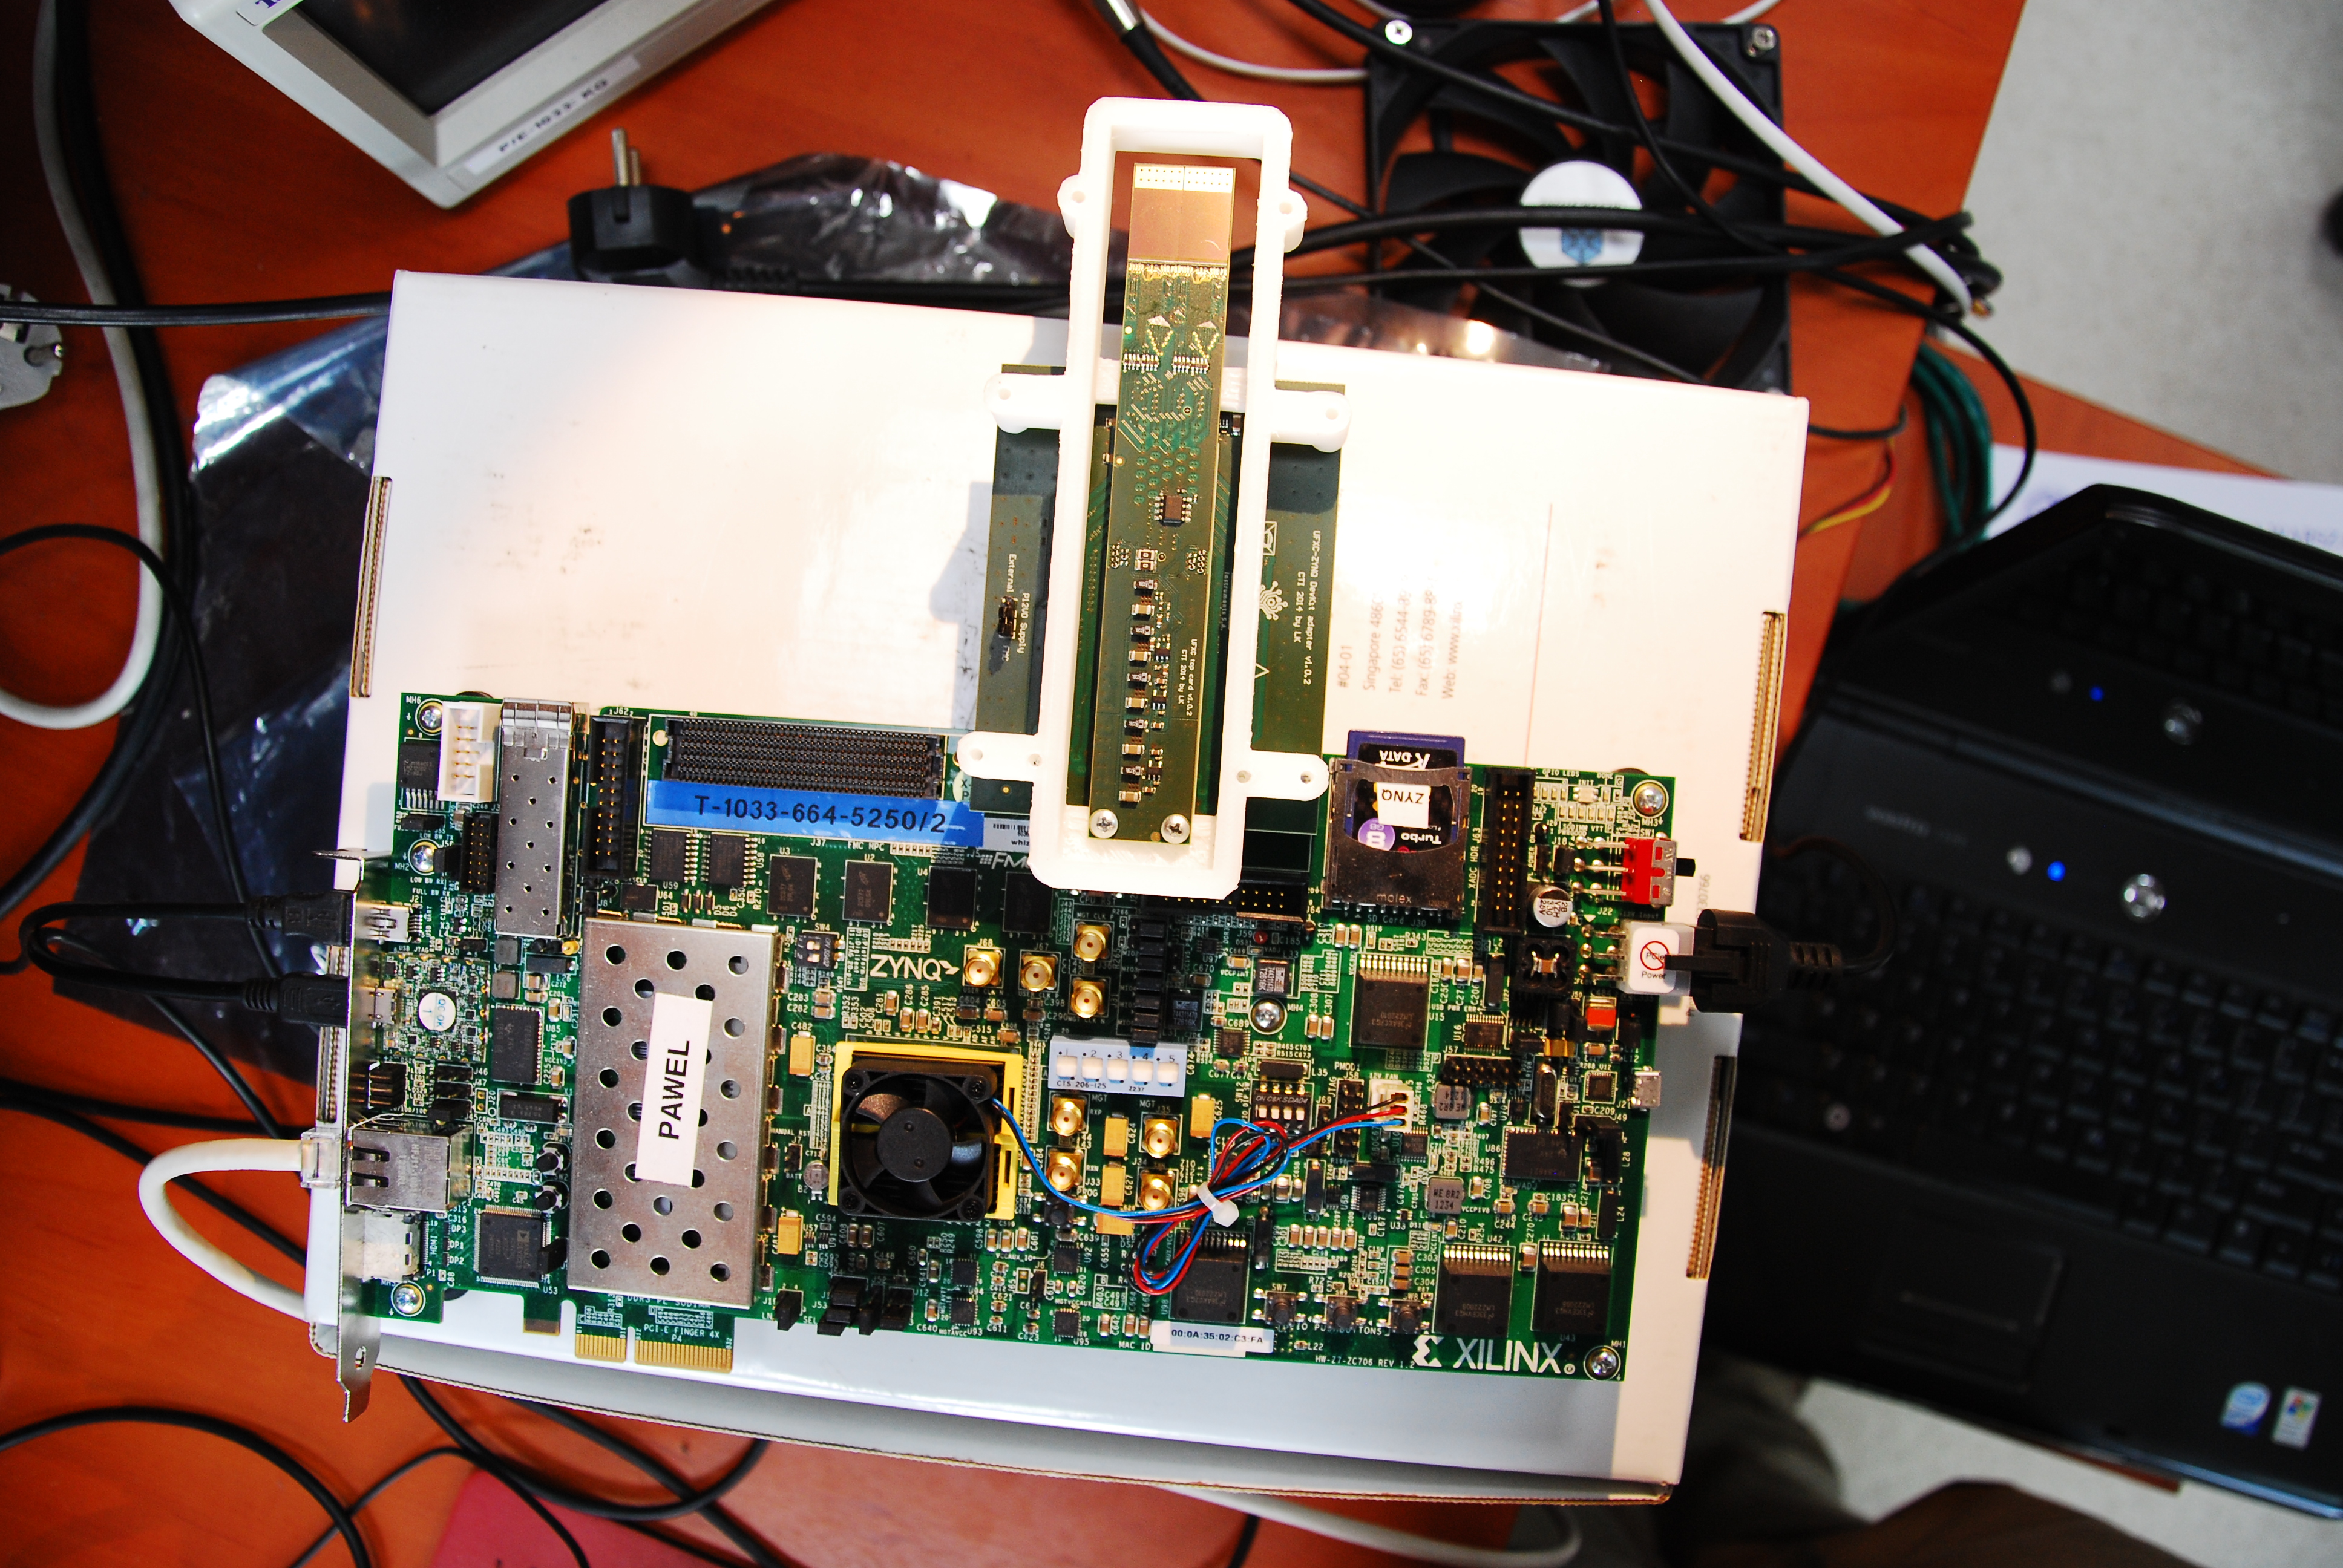
\includegraphics[width=13cm]{img/realisation/zc706_counting.JPG}
%    \caption{Camera Framework design development setup with counting sensor}
%    \label{FIG:DEV_SETUP2}
%\end{figure}
%
%
%\subsection{Xilinx Development Board ZC706}
%
%Xilinx ZC706~\cite{XIL:ZC706} development board with Zynq 7000 Z7045 in FFG900 package is the most advanced development 
%board with Zynq SoC on the market. It has been chosen because it is the largest version of Zynq (Z7045), as well as
%the availability of SFP, FMC and PCIe connectors. The parameters of the board are shown in table\ref{tab:zc706_char}. 
%%
%%\begin{figure}[!h]
%%    \centering
%%    \includegraphics[width=13cm]{img/realisation/zc706-base-board.jpg}
%%    \caption{Xilinx ZC706 Development board}
%%    \label{fig:ZC706}
%%\end{figure}
%%
%
%
%\begin{table}
%    %    \centering
%    \caption{Development board characteristics}
%    \scalebox{0.9}{ 
%        \begin{tabularx}{\textwidth}{|c|X|}
%        \hline
%        \textbf{Subsystem} & \textbf{Characteristics} \\
%        \hline
%        \hline
%        Booting sources & \vspace{0.2cm} \begin{itemize}
%                               \item 2X16MB Quad SPI Flash  
%                               \item SD Card (SDIO interface) 
%                               \item JTAG 
%                           \end{itemize}\\
%       
%
%        \hline
%       Memory &        \vspace{0.2cm} \begin{itemize}
%                              \item DDR3 Component Memory 1GB (PS)
%                              \item DDR3 SODIM Memory 1GB (PL)
%                              \item 2X16MB Quad SPI Flash
%                              \item I2C - 1 KB EEPROM
%                          \end{itemize}\\
%
%
%        \hline
%        Integrated booting sources &         \vspace{0.2cm} \begin{itemize}
%                                                \item 2X16MB Quad SPI Flash  
%                                                \item SD Card (SDIO interface) 
%                                                \item JTAG 
%                                            \end{itemize}\\
%        \hline
%        Memory &         \vspace{0.2cm} \begin{itemize}
%                            \item DDR3 Component Memory 1GB (PS)
%                            \item DDR3 SODIM Memory 1GB (PL)
%                            \item 2X16MB Quad SPI Flash
%                            \item I2C - 1 KB EEPROM
%                        \end{itemize}\\
%
%        \hline
%        Input/Output interfaces &       \vspace{0.2cm}  \begin{itemize}
%                                            \item PCIe Gen2 x4
%                                            \item SFP+ and SMA Pairs
%                                            \item GigE RGMII Ethernet (PS)
%                                            \item 1 CAN with Wake on CAN (PS)
%                                            \item USB OTG 1 (PS) - Host USB
%                                            \item IIC Bus Headers/HUB (PS)
%                                            \item USB UART (PS)
%                                        \end{itemize}\\
%
%        \hline
%         Video components  &   \vspace{0.2cm} \begin{itemize}
%                                            \item HDMI 8 color RGB 4.4.4 1080P-60 OUT
%                                            \item HDMI IN 8 color RGB 4.4.4
%                                        \end{itemize}\\
%
%
%        \hline
%        Connectors &   \vspace{0.2cm}   \begin{itemize}
%                              \item FMC LPC 
%                              \item FMC HPC
%                              \item PS and PL pins on IDC connector (9) 
%                              \item USB OTG 1 (PS) - Host USB
%                              \item IIC Bus Headers/HUB (PS)
%                              \item USB UART (PS)
%                          \end{itemize}\\
%        
%        \hline
%        
%        Clock signals &  \vspace{0.2cm}
%                          \begin{itemize}
%                              \item 33MHz PS System Clock	
%                              \item 200MHz Oscillator 
%                              \item SMA connector connected to FPGA clock input
%                              \item GTX clock signal (156.25 MHz)  
%                              \item OBSAI/CPRI – SFP+ 
%                              \item EXT Config CLK
%                          \end{itemize}\\
% 
%        \hline
%    \end{tabularx}
%    }
%    \label{tab:zc706_char}
%\end{table}
%
%\subsection{CMOSIS CMV4000 CMOS Sensor}
%CMV4000 was briefly described in Chapter 3~[\ref{CH3:CMV}]. The sensor used in the project was attached to an FMC Adapter
%which could be connected to an ZC706 Evaluation board. The module consists of a level shifter for the SPI bus, which is
%CMOS 2.5 V and converts it to CMOS 3.3 V so that it can work properly with Xilinx Zynq on ZC706.  
%
%CMV4000 CMOSIS sensor signals are listed below: 
%
%Inputs:
%\begin{itemize}
%    \item SPI Interface 
%    \item Pixel Clock (up to 440 MHz) 
%    \item Frame Acquisition signal
%\end{itemize}
%
%
%Outputs:
%\begin{itemize}
%    \item 16 DDR data lines 
%    \item Frame valid signal 
%    \item Pixel valid signal
%    \item Return clock signal
%\end{itemize}
%
%Sent data are divided into separate frames which can be acquired by a VDMA mechanism in FPGA logic. This eases the
%development and processing of the incoming data.  
%
%\begin{figure}[h!]
%  \centering
%  \includegraphics[width=13cm]{img/realisation/cmv4000_diag.png}
%  \caption{CMV4000 CMOS Sensor signals}
%  \label{FIG:CMV4000_signals}
%\end{figure}
%
%
%
%\subsection{Counting Sensor}
%A silicon counting sensor is used as another reference sensor for the readout design for the camera framework.
%The sensor consists of a matrix of pixels which count the number of photons of a specific wavelength, and this value can be
%retrieved using a high speed digital interface. The main difference is the fact that the
%sensor does not provide a pixel and frame clock signal, but generates it based on the one that it is driven with. 
%This is a major change compared to a CMV4000 CMOS sensor and presents a different approach to readout. It is also worth
%noting that a
%counting sensor is a \emph{detector} that can be driven continuously, which also makes the readout more complicated.  
%
%Silicon sensor signals are listed below\ref{FIG:COUNTING_SIGNALS}: 
%
%Inputs:
%\begin{itemize}
%    \item Pixel clock signal (up to 500 MHz) 
%    \item Clock signal - for configuration shift register 
%    \item Serial data in - a configuration shift register input
%    \item Strobe - dummy signal 
%    \item Write control - signal latching the new frame 
%\end{itemize}
%
%Outputs:
%\begin{itemize}
%    \item 8 DDR data lines 
%    \item Data Valid 
%\end{itemize}
%
%\begin{figure}[h!]
%  \centering
%  \includegraphics[width=13cm]{img/realisation/counting.png}
%  \caption{Counting sensor signals}
%  \label{FIG:COUNTING_SIGNALS}
%\end{figure}
%
%
%
%\subsection{Samsung 840 250 GB SSD}
%In order to test the Serial ATA interface two Samsung 840 Solid State Drives are used. They are connected to the edge
%PCIe connector on the ZC706 evaluation board. These SSDs use Serial ATA II which allows for 2.5 Gbps of throughput.  
%
%
%\subsection{Workstation PC }
%
%As a main development and testing device, a Dell T7500~\cite{WWW:T7500} Workstation was used. 
%%Figure~\ref{FIG:T7500} presents the computer. 
%
%%j\begin{figure}[!h]
%%  \centering
%%  \includegraphics[width=13cm]{img/realisation/t7500.jpg}
%%  \caption{Dell T7500 Workstation PC}
%%  \label{FIG:T7500}
%%\end{figure}
%
%Dell T7500 Workstation parts are listed below:
%\begin{itemize}
%    \item Intel Xeon E5 CPU
%    \item NVIDIA Tesla 2050 
%    \item 12 GB of DDR3 RAM
%    \item Intel 10/100/1000 Ethernet Card
%\end{itemize}
%
%During the project development the following tools and software were used:
%
%\begin{itemize}
%    \item Xilinx Vivado 2014.4 Design Edition with patch~\cite{xil:patch}
%    \item Xilinx Petalinux 2014.4
%    \item gcc-4.8
%    \item iSim simulator for Vivado
%    \item PC with CentOS 7 x86\_64\footnote{Officially supported OS by Xilinx.}
%\end{itemize}
%
%
%
%
%%. The sensor is placed on a dedicated FMC card
%%connected to the development board. Figure~\ref(fig:zc706)  And as you can see in the picture I have tested the SATA interface (cause the discs are connected) as well as Ethernet connection via SFP transceiver
%%(1 Gbps or 10 Gbps Ethernet).
%%
%%I think that the best way to describe how does my system work it to start from the sensor and then go all the way to 
%%the gigabit interface. 
%
%
%%\section{Basics of Embedded System Design on Xilinx Zynq SoC}
%%\label{ch3_realisation:basics}
%%block diagram
%%add a counter to the Zynq to the axi and couple of registers
%%export to sdk
%%write hello world
%%compile run execute
%%design linux run and access the register under the general io driver
%
%%  \subsubsection{Creating project}
%%  In order to create the project, one has to use a tool \textbf{petalinux-create} which creates the project in a
%%  specified folder with default configuration. 
%%
%%  %TODO: Add listing of the petalinux create commnad>
%% 
%%\begin{lstlisting}
%%    $pzdunek:$ petalinux-create -n camera_framework
%%\end{lstlisting}
%
%
%%\section{System architecture design}
%
%%\emph{Universal camera framework} consists of a digital system, firmware and software running on Xilinx Zynq SoC.
%%In order to explain the realisation of the project one has to understand the every aspect of design. For this reason,
%%first, an introduction to embedded system design using Zynq SoC will be presented and afterwards the camera framework
%%design. 
%
%%\section{Basics of Embedded System Design on Xilinx Zynq SoC}
%%\label{ch3_realisation:basics}
%
%%\section{Base Universal Camera Framework Design}
%%based on TRD given by Xilinx
%%Zynq configuration
%%   peripherals
%%   MIO
%%   Address space
%%    
%% adding IP Cores and configuration and simulations
%% tests on baremetal
%% 
%%    
%
%%\subsection{Lens}
%
%%\section{Firmware}
%
%%This section presents the realisation of the firmware for the camera framework. 
%
%%The firmware is divided into following parts:
%
%%\begin{itemize}
%%  \item{Operating System architecture}
%%  Configuration of Petalinux Operating Sytem and FreeRTOS in Assymetric Multiprocessing nad Symmetric Multirpocessing
%%  scenario is presented as well as description of the internal data handling and communication between the operating systems.  
%%  \item{Linux firmware}
%%  Linux firmware consits of program which are run on the Petalinux OS which control the digital system using Universal
%%  Input Output driver and also general purpose programs like \textbf{ptpd} which allows for achieving PTP
%%  synchronisation over Ethernet. Additionally, a number of configuration scripts are presented which were necessary for
%%  the whole firmware to run correctly. 
%%  \item{FreeRTOS firmware}
%%  Firmware on RTOS is used for configuring the registers responsible for controlling the camera. A description of tasks
%%  is presented and explained. 
%%  \item{Baremetal testing firmware}
%%  The development of final control programs on Embedded Linux or FreeRTOS is superceded by testing it on Zynq's Cortex
%%  A9 MPCore in Baremetal configuration. 
%%\end{itemize}
%
%%First an architecture of the operating system is presented. Then the applications running on Linux operating system
%%are described. In the end the FreeRTOS is shown and baremetal 
%
%
%\section{System architecture}
%%System architecture diagram
%%
%%System hardware diagram
%%
%%System firmware diagram 
%Having specified the set of requirements, a final system architecture is designed which will be a foundation for
%developing the camera framework~\cite{BOOK:MAKING_EMBEDDED}. The architecture consists of: firmware, digital
%system and software. 
%
%
%\subsection{Firmware}
%The firmware for the camera can run as an independent Linux Embedded operating system run on two cores or as a hybrid 
%solution where one core runs Xilinx Petalinux OS and the other one is running FreeRTOS. A double solution is proposed
%due to the fact that some applications don't require the use of a Real-Time Operating System and also the
%communication between the cores using the vendor proposed method with \textit{rpmsg} system~\cite{XIL:AMP_LINUX_FREERTOS}
%does not work properly. Therefore a simple message passing using embedded OCM\footnote{On-Chip Memory} has to be developed and its
%performance is limited.  
%
%The creation and configuration of the Petalinux Embedded OS and its applications is described in more detail in the
%following sections of the chapter, as well as the design of the FreeRTOS. 
%
%One aspect of camera design was the testing of the digital system. As far as embedded system design is concerned the
%most efficient way to test the designed IP's from software is using as simple software as possible, to be sure
%that any errors that happen during development are not caused by software. For this reason the \textit{Baremetal
%firmware} is also presented, in order to show how the testing was performed. 
%
%\subsection{Digital system}
%
%The design of any digital system is a complicated process, due to the architecture of FPGA.
%Digital Systems designers need to take into account not only the functional behaviour of the system being designed, but
%also the timing relationships between the different parts and internal blocks.   
%Xilinx proposes the use of its methodology \textit{Ultra-fast embedded system design}~\cite{XIL:ULTRA_FAST} with accompanying
%checkbox application, so that one can make sure that he is doing everything properly. On one side this approach is highly recommended due to
%the fact that each critical part of the design is being done step-by-step and it is known by whom and when it was done. 
%On the other side it is more targeted for larger teams than for single or small teams of designers. For this reason the 
%methodology for the design of the digital system in the camera system called for the basic system (consisting 
%of Zynq SoC configuration and few IP Cores) to be designed first.\\ 
%
%Firstly, the simple system was fully verified and the basic software was written. After a successful deployment of this 
%basic structure, the more complex IPs have been developed, tested and then incorporated to the design. 
%This iterative approach is a natural way of developing any engineering system~\cite{CIT:KENT_BACK}.  
%
%The digital system in the camera framework consists of a few main IPs:
%
%\begin{itemize}
%    \item CMV4000 video data acquisition
%    \item Counting sensor video data acquisition
%    \item PCS/PMA 1 GbE IP Core
%    \item Serial ATA Core
%\end{itemize}
%
%The design of the control over those IPs, as well as modifications that were performed, are described in the following
%sections. 
%
%\subsection{Software}
%
%The control of the camera system is performed by an external PC which communicates with the camera through Ethernet. 
%For this reason, an application had to be developed in order to control the camera. The application was written in C.
%It uses \textit{IP Sockets} for communication with the server running on the camera's embedded Linux. 
%
%%with the use of \textif{pyScaffold}~\cite{WWW:PYSCAFFOLD} framework.
%
%%TODO Add nice block diagram PC + dev board, senosr
%
%%\begin{figure}[!h]
%%    \centering
%%    \includegraphics[width=13cm]{img/realisation/sys_diag.png}
%%    \caption{Camera framework detailed system diagram}
%%    \label{FIG:SYS_DIAG}
%%\end{figure}
%%
%%
%
%\section{Camera operating system}
%
%\subsection{Petalinux Embedded Linux}
%
%The embedded operating system running on the camera is a Xilinx distribution of Linux: Petalinux \cite{XIL:PETALINUX}.
%The Petalinux system provides an easy way to configure and setup an operating system for Zynq SoC and also for Microblaze. 
%The configuration is done using a set of tools provided by the vendor. On the one hand, Petalinux makes it possible to
% quickly design a system, but on the other it makes it less versatile and flexible. 
%
%What is essential is that Petalinux kernel provides a set of drivers and programs dedicated specifically for Zynq SoC. 
%These drivers make it possible to easily use IP Cores added to Programmable Logic from Linux OS. Additionally, an
%automatic \textit{Device-Tree} generation is also performed, which takes into account the added IP Cores to the digital
%system.  
%
%Petalinux generates the following files which are then used as a system image: 
%\begin{itemize}
%    \item \textbf{FSBL} - first stage bootloader - which is a baremetal ARM A9 application which sets all the necessary
%        configurations such as boot source during runtime 
%    \item \textbf{uboot} - a Linux bootloader
%    \item \textbf{image.ub} - system image 
%    \item \textbf{bitstream.bit} - a bitstream file for FPGA configuration
%\end{itemize}
%
%The FSBL and \textit{ps\_init} files are automatically generated with the petalinux project. It is worth noting that configuration of
%peripherals before Linux boot can be performed only if the booting of the system is being done either using SD Card or
%Flash memory. It cannot be performed by booting the system through JTAG due to a different order of loading system image
%and bitstream. 
%
%Another key aspect of Petalinux is that it is based on \textit{yocto}~\cite{WWW:YOCTO}, which is an alternative to
%\textit{buildroot} embedded Linux system design platform. This makes it easier to adjust and modify based on yocto
%documentation.   
%
%\subsubsection{Configuration}
%
%First of all, IP core configuration in Block Design is exported to HDF\footnote{Hardware Description File}. 
%This file is put into the Petalinux project in order for the tools to create the configuration for the OS based on 
%what has been designed in Programmable Logic. This is done using  \textbf{petalinux-config} 
%program with option \textbf{--get\_hw\_description} flag. An example of the full command is listed below.  
%
%\begin{lstlisting}
%pzdunek$zdunek:~$ petalinux-config --get-hw-description=. 
%\end{lstlisting}
%
%%\subsubsection{Main configuration}
%
%The next step of creating the Petalinux OS is the configuration of specific parts of the system:kernel, bootloader
%and rootfs. The main configuration of Petalinux is done using the \textbf{petalinux-config} command. 
%%
%%\begin{figure}[H]
%%    \centering
%%    \includegraphics[width=13cm]{img/realisation/petalinux_config.png}
%%    \caption{Configuration window of petalinux-config program}
%%    \label{fig:petalinux_config}
%%\end{figure}
%
%
%This configuration program allows for choosing a specific kernel, bootloader, rootfs and also the place in address
%space of each component. For this camera project, a specific version of kernel was used in order for PCS/PMA IP Core
%to work. This setting is done in accordance to Xilinx Application Note~\cite{XIL:ZYNQ_PL_ETH}.
%Figure~\ref{fig:petalinux_config_kernel_1} presents an example of configuration setup screen. 
%
%\begin{figure}[h!]
%    \centering
%    \includegraphics[width=13cm]{img/realisation/petalinux_config2.png}
%    \caption{Configuration of Kernel source}
%    \label{fig:petalinux_config_kernel_1}
%\end{figure}
%
%
%\paragraph{Kernel}\mbox{}\\
%
%In order to configure the Kernel, the designer has to use \textbf{petalinux-config} program with option \textbf{ -c
%    kernel}. The following options were selected in the kernel configuration: 
%
%\begin{itemize}
%    \item kernel set to remote (for PCS/PMA IP Core)
%    \item early kernel error messages on (EARLYPRINTK=y)
%    \item added support for REMOTEPROC and RPMSG for multicore communication
%    \item UART1 is set as standard output
%\end{itemize}
%    
%%    Figure~\ref{fig:petalinux_kernel_config} presents the main windows of the configuration. 
%%    Listings~\ref{lst:sysconf},~\ref{lst:remote_set} present the main options set for the kernel. 
%
%%\begin{figure}[H]
%%    \centering
%%    \includegraphics[width=13cm]{img/realisation/petalinux_config_kernel.png}
%%    \caption{Kernel configuration}
%%    \label{fig:petalinux_kernel_config}
%%\end{figure}
%
%\paragraph{Rootfs}\mbox{}\\
%In order to configure the \emph{rootfs}, the designer has to use \textbf{petalinux-config} program with option \textbf{ -c
%    rootfs}. The following options were selected in the rootfs configuration: 
%\begin{itemize}
%    \item packages installed: busybox, gdbserver, libc6, libgcc, libstdcplusplus\_dev,libthread\_db1,libc\_headers
%    \item tools: i2c, ifupdown,initiscripts,tcf\_agnet, dropbear, ethtool, openssh, tcpdump, strace
%    \item applications: autologin, blockram, initial\_setup, si570, socket\_server 
%\end{itemize}
%
%One important aspect of the rootfs configuration is that the \textit{applications} can also be added using Petalinux
%\textbf{-create} program. It automatically creates a simple C based application and adds it for selection to rootfs
%configuration. This program is assigned a priority during runtime using \textbf{init.d} daemon. The created application
%can be customised to the needed requirements, and this was done in the project. The custom applications were:
%
%\begin{itemize}
%    \item \textbf{autologin} - a program which automatically logs in a user to the camera (this was needed in order for the PCS/PMA
%        driver to be loaded)
%    \item \textbf{blockram} - an application which is used to read and write to and from a blockram to configure the IP Core for
%        silicon counting sensor
%    \item \textbf{initial\_setup} - a program for setting general parameters at boot time 
%    \item \textbf{si570} - a program which changed the frequency of the SI570 oscillator at the boot time
%    \item \textbf{socket\_server} - a main camera server program used for receiving the commands through Ethernet and executing
%        them
%\end{itemize}
%
%For the selection of command line programs, \emph{busybox} is used. Due to the fact that applications are run on the 
%camera system, it is useful to have some kind of debugging
%capability, and for this reason C/C++ development and debug libraries and programs were added. 
%%
%Selected programs are some of the most commonly used in embedded Linux systems. 
%\textit{TCF\_AGENT} application is less widely known. This program is used for online debugging of Linux applications 
%running on Zynq Cortex A9 MPCore using \textit{XSDK}. This process is explained more in the debugging section~\ref{CH5:DEBUGGING}.
%
%%\paragraph{General Petalinux Configurations}
%%Some additional options were set in the Petalinux-configuration:
%%\begin{itemize}
%%    \item root password set = "camera"
%%    \item services configuration: inetd\_fptd, inetd\_telnetd
%%    \item user debugging turnet on
%%\end{itemize}
%
%
%
%%Listings below~\ref{list:petalinux_rootfs_config},~\ref{list:petalinux_rootfs_config1},~\ref{list:petalinux_rootfs_config2} presents the main set options for the kernel. 
%
%%\begin{figure}[H]
%%    \centering
%%    \includegraphics[width=13cm]{img/realisation/petalinux_config_rootfs.png}
%%    \caption{Kernel configuration}
%%    \label{fig:petalinux_rootfs_config}
%%\end{figure}
%
%%\subsection{Summary}
%%
%%The main aspects of the Petlinux operating systems are listed below. The detailed list of kernel and rootfs
%%configuration can be found in the project files of the Petalinux attached to this thesis. 
%%
%%\begin{itemize}
%%    \item kernel set to remote (for PCS/PMA~\ref{CH5:PCS_PMA})
%%    \item early kernel error messages on (EARLYPRINTK=y)
%%    \item added support for REMOTEPROC and RPMSG for multicore communication
%%    \item advanced rootfs setup
%%
%%        \begin{itemize}
%%            \item packages intalled: busybox, gdbserver, libc6, libgcc, libstdcplusplus\_dev,libthread\_db1,libc\_headers
%%            \item tools: i2c, ifupdown,initiscripts,tcf\_agnet, dropbear, ethtool, openssh, tcpdump, strace
%%            \item applications: autologin, blockram, initial\_setup, si570, socket\_server 
%%        \end{itemize}
%%\end{itemize}
%
%
%%An exact \textit{defconfig} file with the Kernel configuration can be found in the Appendix \ref{app:defconfig}.
%
%%Listing~\ref{lst:sysconf} presents the \emph{Linux Components Selection} part of the configuration. As it can be
%%seen the FSBL and \textit{ps\_init} files are automatically generated with the petalinux project. It is worth noting that configuration of
%%peripherals before Linux boot can be performed if certain design desicions are made, as described in the
%%section~\ref{chap:periph_conf} and in the appendix~\ref{apndx:ZynqProjectTips}. What is important is that the kernel
%%is set as a remote source. This is done due to the use of \textbf{Xilinx PCS/PMA 1 GbE IP Core}.
%%
%
%%Listing~\ref{list:petalinux_rootfs_config} shows the main configuraion of the rootfs for Petalinux. As it can be
%%seen the advanced configuration mode is selected. For the selection of command line programs \emph{busybox} is used.
%%Due to the fact that applications are run on the camera system, it is useful to have some kind of debugging
%%capability, and for this reason C/C++ development and debug libraries and programs were added. 
%%
%%Listing~\ref{list:petalinux_rootfs_config1} presents the added programs to the rootfs. Most of them are commonly
%%used in many embedded linux applications. \textit{TCF\_AGENT} application is less widely known.
%%This program is used for online debuging of Linux applications running on Zynq Cortex A9 MPCore using \textit{XSDK}. 
%%This process is more explained in the debugging section~\ref{chap3:debugging}.
%
%\subsubsection{Applications}
%The most important applications are described in more detail in the following paragraphs. 
%
%
%\paragraph{Camera server}\mbox{}\\
%
%The camera server application is the main program running on the camera. Mgr inż. Maciej Trochimiuk was mainly
%responsible for the development of the application. It was written in C and performed the
%following functions:
%
%\begin{itemize}
%    \item control the digital system with the use of registers connected to AXI General Purpose bus 
%    \item receive and transmit data and commands over Ethernet
%\end{itemize}
%
%%\begin{figure}[H]
%%  \centering
%%  \includegraphics[width=13cm]{img/realisation/camera-server-application.png}
%%  \caption{Camera server application block diagram}
%%  \label{fig:camera_server}
%%\end{figure}
%
%
%The control over digital system is done using UIO (Universal IO) userspace driver which allows for direct read and write
%to physical memory address. In order to do that, first an IP Core has to be connected to an AXI General Purpose
%Bus, which allows the Processing System to map the IP Core's register to specific addresses in address space. Then, the
%Device Tree has to be properly setup so that the operating system knows where exactly in the memory the registers of the IP
%Cores are stored and what the address range is. 
%
%%This is explained in detail is the Configuration of Operating System
%%subsection and control register configuration in digital system design section.   
%
%The Ethernet communication is being done using TCP/IP Sockets~\cite{WWW:TCP_IP_SOCKETS}. Three different ports are used for 
%communication between PC and camera server: 
%\begin{itemize}
%    \item \textbf{Data Port} - for sending video data from camera to PC (UDP)
%    \item \textbf{Control Port} - for sending commands from PC to camera server (TCP/IP)
%    \item \textbf{Maintenance Port} - for sending log messages from camera to PC (TCP/IP) 
%\end{itemize}
%
%This way, the different functionality is separated between different ports, which eases the development. 
%
%%move to other section about synchronisation? TODO
%
%\paragraph{ptpd}\mbox{}\\
%
%In order to achieve synchronisation over Ethernet protocol, a \textbf{ptpd} application was tested on the camera framework. 
%\textbf{ptpd} is a daemon program which adds support for the IEEE 1588v2~\cite{NIST:PTP}~\cite{LINUX:PTP} in Ethernet networks, provided that
%MAC\footnote{Media Access Controller} supports it. This allows for \emph{ms} range synchronisation over the Ethernet.
%Xilinx has provided an application note describing the use of the \textbf{ptpd} daemon on Zynq SoC~\cite{XILINX:PTPD}. 
%  
%
%In the case of camera framework, a test setup was performed where two ZC706 development boards were connected to each other
%and a \textit{master - slave} PTP synchronisation test was performed. The development boards were running custom
%Petalinux designed for camera framework and the Ethernet access was provided using PCS/PMA 1 GbE IP Core. 
%
%The test of synchronisation was successful between two modules with achieved synchronisation in a \textit{ms} range. 
%\textbf{ptpd} daemon can be used in any application running on the camera, provided that the network supports 1 GbE PTP.
%The only limitation of the synchronisation is the requirement of having a PTP-Master supporting 1 GbE networks. 
%
%
%\paragraph{Autologin application}\mbox{}\\
%%TODO Change font to normal courier
%
%This application logs in to the camera after a proper booting process is performed. This was required in order to
%properly load the PCS/PMA IP Core driver. The application executes an \textbf{exec} function during the execution of
%\textbf{init} scripts. 
%
%\paragraph{PCS/PMA IP Core driver setup}\mbox{}\\
%
%PCS/PMA IP Core Driver is used in order for the Ethernet to work in the Camera framework. 
%
%%    \subsubsection{Main application - \textbf{camera-server}}
%
%Initial setup script that is run at the beginning of the boot sequence provides default configuration for
%the device. The script is created as a petalinux application with redefined configuration. The change had to be
%made so that the script is added to each iteration of petalinux building. Listing [\ref{APP:PCS_PMA}] shows the
%written script for the initialization of the PCS/PMA Ethernet module. First, it finds the module in the kernel path
%and then loads it. An exact path cannot be specified because with each clean-up of the petalinux project, a new
%kernel hash is downloaded from the repository as per the configuration. In order to overcome this issue, a
%find function of bash has been used. 
%
%A \emph{~/.profile} file is created after loading the kernel module which
%is used to pre-configure Ethernet setup. The petalinux is specific about the Ethernet connection and for
%undiscovered reason, the Ethernet interface did not work when the user is not logged in. For this reason another
%application was written which automatically logs in the root user. One has to bear in mind that this solution is
%not safe, and another user should be created in order to perform this configuration. Nevertheless, this solution
%is acceptable from the development point of view. After the root user is logged, a prompt message is 
%printed out and also the Ethernet interface is brought up with the \textbf{ifconfig} command.   
%
%
%\subsubsection{OS boot}
%There are multiple ways of booting the Xilinx Zynq SoC~\cite{WWW:XIL_BOOT} including: SD Card, NOR Flash, Ethernet, PCI
%Express and JTAG. The booting procedure used in this project was SD Card boot and JTAG boot during development. 
%
%Boot process of the Processing System\ref{FIG:BOOT} is performed after the \textit{PS\_POR\_B} reset pin de-asserts. Depending on
%the configuration of the dedicated boot pins the Bootloader is executed from embedded BootROM code in the on-chip
%ROM of the processor~\cite[Section 6.1]{DSH:TRM}. 
%
%\begin{figure}[h!]
%    \centering
%    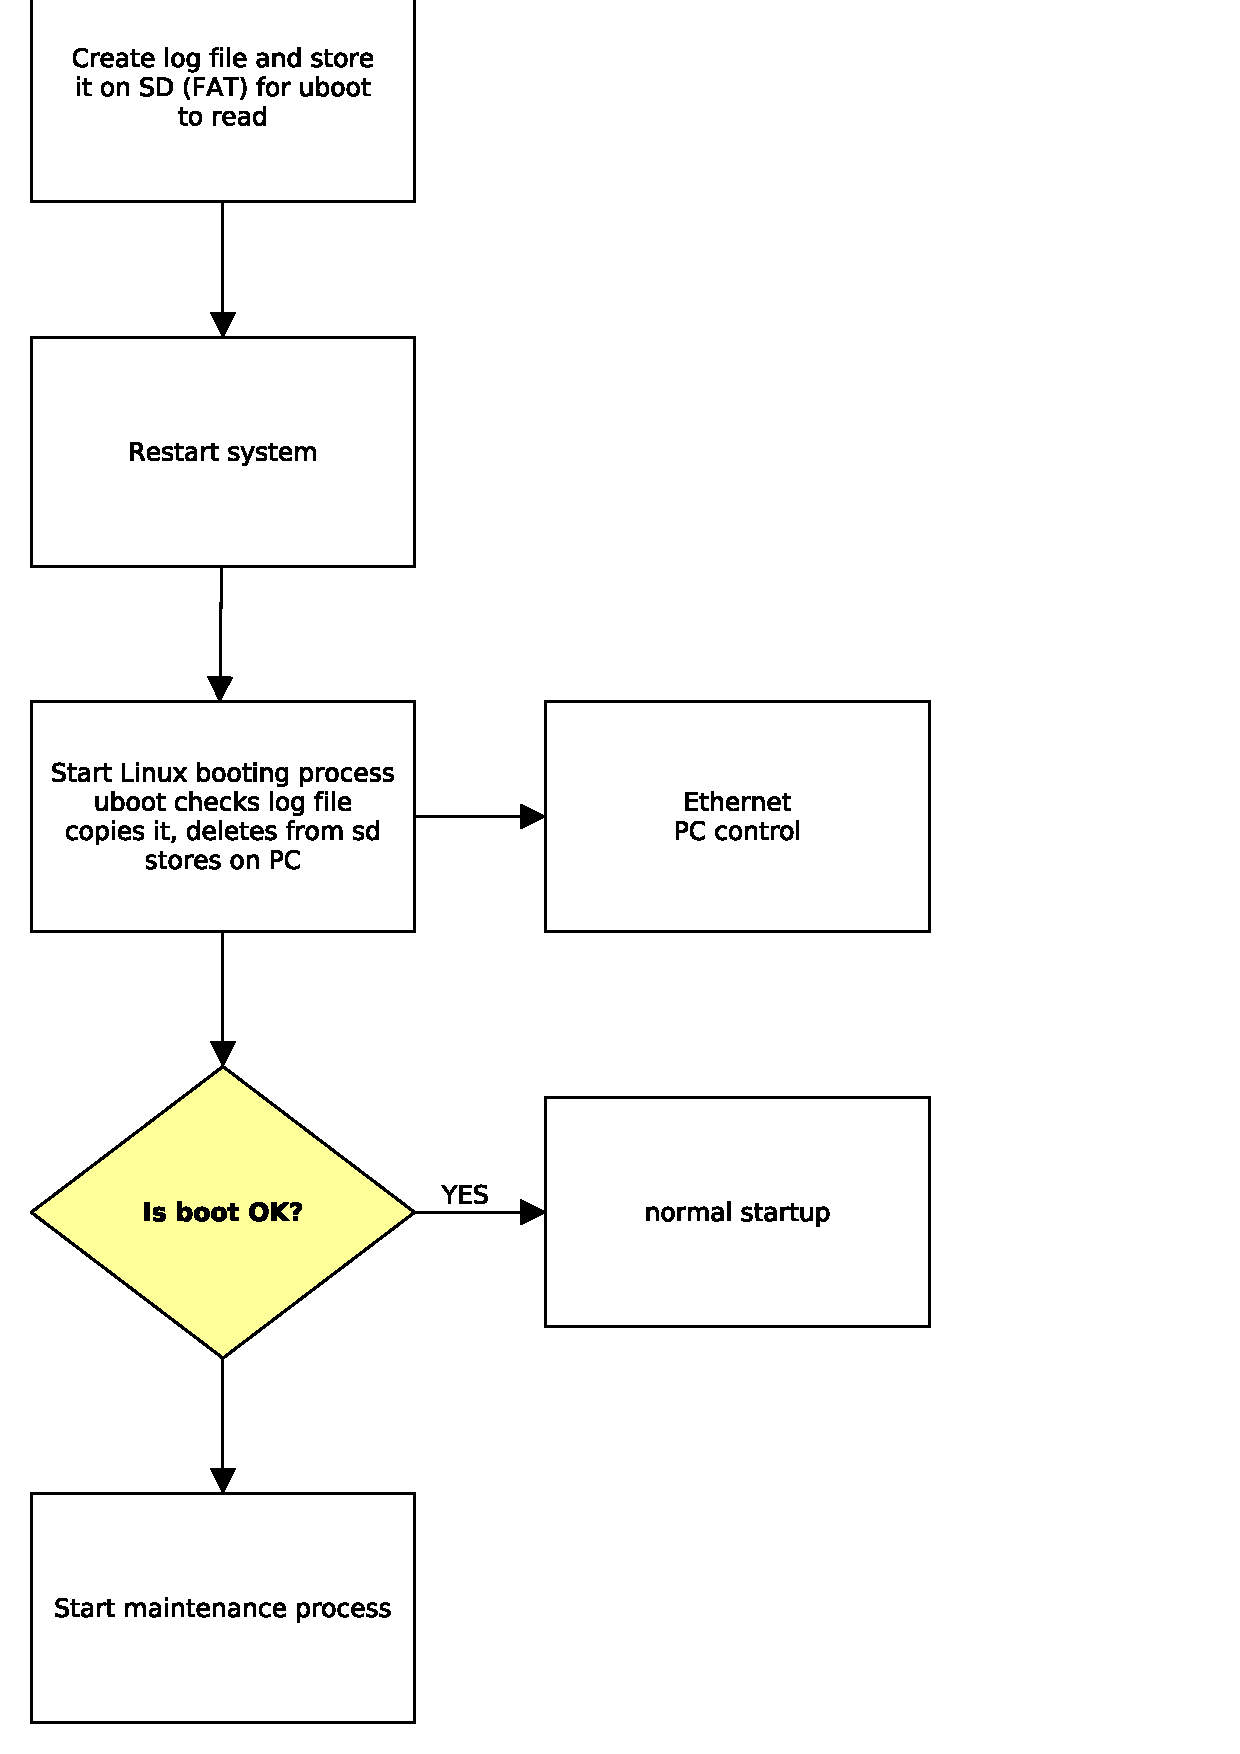
\includegraphics[width=10cm]{./img/realisation/boot.png}
%    \caption{System boot process diagram}
%    \label{FIG:BOOT}
%\end{figure}
%
%
%\paragraph{JTAG boot}\mbox{}\\
%Booting can be performed by JTAG interface, which is particularly useful during development. A \textbf{petalinux-boot}
%supports a command \textbf{-jtag} which boots the operating system and loads the bitstream via JTAG. One has to bear in mind that the
%procedure has a \emph{different} sequence than the SD Card boot - the bitstream is loaded before the OS. In this case one
%cannot rely on any configured peripherals during the boot (e.g. I2C configurable oscillator).    
%
%Xilinx Zynq allows for the use of I2C and other peripherals during the boot without the need for Programmable Logic, but
%this is constrained to specific pins on the IC and a designer has to make sure to specifically use them and not the ones
%connected via MIO reconfigurable matrix (which works after the FPGA is configured).
%
%
%\paragraph{Standard boot}\mbox{}\\
%Standard boot process is performed from an SD Card.  
%
%SD Card contains a set of files which are loaded after boot of the Processing System: 
%
%\begin{itemize}
%    \item BOOT.bin
%    \item image.ub
%\end{itemize}
%
%BOOT.bin is a file containing the boot image which is also a set of files:
%
%\begin{itemize}
%    %  \item a BIF file (Boot Information File) 
%    \item fsbl.elf - First Stage Bootloader application
%    \item bitstream.bit - bitstream for Programmable Logic
%    \item uboot.elf - higher level bootloader
%\end{itemize}
%
%Whereas image.ub contains the Kernel, Device Tree Blob and minimal root file system for Petalinux. 
%
%Both of those files are created during configuration of Petalinux Operating System. The configuration of all the
%parts of the OS can be customized, e.g. by adding your own applications which will be executed at a runtime.
%
%
%\subsubsection{Bootloader - Uboot}
%The bootloader used in the project is Uboot (Universal Bootloader) which is commonly used in embedded system using
%Embedded Linux~\cite{WWW:UBOOT1}~\cite{WWW:UBOOT2}.  
%
%The configuration of Uboot is unchanged. 
%
%
%\subsubsection{Device Tree}

%\emph{A device tree is a data structure describing hardware}~\cite{WWW:LINARO}. Embedded Linux uses a Device Tree Blob 
%as a reference for the peripherals. It contains information regarding the physical address and the driver name for
%specific devices~\cite{LNX:DEVICE_TREE}~\cite{XIL:DEVICE_TREE}. The introduction of a Device Tree Blob has made the
%creation of operating systems more 
%flexible, especially for embedded systems using SoCs where the configuration of
%the Main Processing Unit may differ greatly from one device to another. There is no need to have scripts initialize 
%the hardware, since everything is done during the boot process.
%
%Listings~\ref{LST:DEVICE_TREE} present the added portion of the device tree apart from the one created automatically by
%the \textbf{petalinux-build} program. Figure~\ref{fig:device_tree_structure} presents the Device Tree structure that is
%used in the Camera System. 
%
%\begin{figure}[h!]
%    \centering
%    \includegraphics[width=10cm]{img/realisation/device_tree_diag.png}
%    \caption{Device Tree structure of a camera system}
%    \label{fig:device_tree_structure}
%\end{figure}
%
%
%% Describe the realization of the framework using ZC706 and then in the test application. Write that you've used the
%% MArek Burza desing and adapted it to ZC706. The readout for CMV4000 was changed so that it can be used in Linux ? 
%% 
%
%
%The main Device Tree file includes the dedicated configuration of the SoC: the address space of dynamic memory,
%configuration of Ethernet MAC (gem1), UART and I2C protocol devices listing. The embedded Device Tree configuration file
%contains more specific configuration - what is connected to AMBA/AHB bus in Programmable Logic. What is worth noting is
%the configuration of the embedded register\ref{LST:REG}. The configuration of an embedded register in Programmable
%Logic sets the address where the register is placed in the physical address space and also that the UIO (User Space
%Input/Output) driver is going to be used for its control. 
%
%The use of UIO greatly simplifies the use of any custom IP Core embedded in Programmable Logic due to the fact that
%there is no need for developing your own driver. UIO drivers allow for direct write and read to specific address memory
%space which, in the case of an embedded register, will set the value of a specific register.  
%
%A device tree is loaded during the system boot by bootloader along with the kernel.  
%
%% \subsubsection{Setup}
%% 
%% \subsubsection{Camera task}
%% 
%% \subsubsection{Focus task}
%%\subsection{Camera functions}
%%
%%\subsubsection{Sensor control}
%%
%%\subsubsection{Data transfer}
%
%\subsection{FreeRTOS}
%This section describes the setup of FreeRTOS operating system on Zynq SoC used in the camera framework development.
%The FreeRTOS was used and tested with the cooperation of CMV4000 IP Core and Serial ATA IP Core and provided information
%regarding the pros and cons of the use of this operating system on the camera. The work described here was based on the work of mgr inż. Marek Burza who has tested the CMV4000 sensor on Zynq Zedboard evaluation board. The further development of the idea was to move the design to ZC706 verify it and add Serial ATA support. 
%
%\subsubsection{Basic information}
%FreeRTOS is a real-time operating system targeted for embedded systems. It is widely supported by many architectures and
%has been developed by an Open-Source community for many years. 
%%TODO: Add FreeRTOS description. 
%
%\subsubsection{FreeRTOS configuration}
%In order to run FreeRTOS on Zynq SoC, a number of steps have to be taken. First of all, one can choose the modified
%version of FreeRTOS provided by Xilinx~\cite{WWW:XIL_FREERTOS} or the one available directly from \url{freertos.org}. 
%
%The advantage of the first is the pre-configured linker scripts as well as few example projects.  
%
%The FreeRTOS sources are added to the project and then using \textbf{XSDK} a full FreeRTOS application can be created.
%There are several crucial aspects of running FreeRTOS on Xilinx Zynq SoC: 
%
%\begin{itemize}
%    \item linker script
%    \item memory regions 
%    \item heap allocation algorithm implementation
%    \item compiler options
%\end{itemize}
%
%\subsubsection{FreeRTOS tests}
%FreeRTOS capabilities were tested for the camera framework by performing the following tests:
%\begin{itemize}
%    \item a FreeRTOS and Baremetal running in AMP Configuration 
%    \item a FreeRTOS and Linux running in AMP Configuration 
%\end{itemize}
%
%These tests were performed to validate the usefulness of FreeRTOS for camera framework.
%
%\paragraph{FreeRTOS and Baremetal}\mbox{}\\
%
%In this configuration FreeRTOS application was run on first core of Cortex-A9 and Baremetal code was run on the second core
%of Cortex-A9. The L2 cache synchronisation between the cores was turned off. FreeRTOS was running several tasks while
%Baremetal code was waiting for an interrupt from the Programmable Logic. This would identify the scenario where FreeRTOS
%is responsible for communication between the PC and the camera and control, whereas Baremetal would function as an
%independent subsystem taking care of video data acquisition. 
%
%The test was run successfully, with simple tasks on FreeRTOS and a timer on Baremetal, proving that this architecture
%can be used for a camera system. One drawback of this idea is that the communication between the FreeRTOS and Baremetal
%is limited by using OCM\footnote{On-Chip Memory}. 
%
%\paragraph{FreeRTOS and Linux}\mbox{}\\
%
%In this configuration Petalinux Embedded OS was run on the first core of Cortex-A9 and FreeRTOS was run on the second core. 
%Petalinux was configured in \textbf{SMP} configuration, but with just one core enabled. During the booting, an
%application is loaded for the second core and is executed by the Linux OS. For this reason, only after a proper
%booting can FreeRTOS perform any critical task. In this configuration, Linux is responsible for control and
%communication and FreeRTOS is responsible for performing real-time tasks.  
%
%The AMP configuration of the operating system on a camera framework was designed with accordance to Xilinx
%documentation~\cite{XIL:AMP_LINUX_FREERTOS}. Basic AMP scenario for Baremetal worked correctly, although  
%the example design with Linux and FreeRTOS could not communicate using \textbf{rpmsg}.
%
%The setup involved performing following steps: 
%
%\begin{itemize}
%    \item running a simple baremetal AMP test
%    \item creating a simple FreeRTOS application
%    \item using a modified FSBL from Xilinx
%    \item modifying compiler flags for FreeRTOS application to:\textit{-g -DUSE\_AMP=2} 
%    \item modifying linker script
%    \item modifying the Petalinux Kernel configuration so that it uses just one CPU:\textit{-MAXCPUS=1}
%    \item adding an application to Petalinux which wakes up the second CPU (CPU1)
%    \item adding rpmsg support to Petalinux
%    \item modifying the linker script so that a special memory region is added for rpmsg data exchange
%    \item turned off cache coherency in L2 cache
%\end{itemize}
%
%All these tasks allowed for running an AMP Configuration of the operating system for the camera framework. Some more
%complicated tasks need to be described in more detail.
%
%%\subsubsection{Second core boot}
%The booting of the second core works differently for different revisions of Zynq SoC. This was one of the main design
%issues during the development of this feature. Initially, the system was developed using ZC706 development board version 1.0
%which uses silicon rev 2.0. Then the design moved to ZC706 version 2.0, which uses silicon revision 3.0. There are some
%differences in the silicon which caused problems. In order to configure the second core so that it is booted by the
%first one (CPU0), the program has to have a simple infinite loop condition at the beginning of \textit{main()} function
%which waits for the change in WFE(\textit{Wait For Event} variable which can be set by the first core (CPU0).
%
%The behaviour of the WFE variable is different for different revisions of Zynq. For older revisions, the second core
%waits for the WFE to change from 0 to 1, whereas on the newer cores it waits for the change from 1 to 0. This crucial
%change which is difficult to understand directly from the documentation caused some problems during development. 
%
%For this reason, the main functionality of the camera framework was designed \emph{solely} for Petalinux and for
%Baremetal. 
%
%%\subsection{Multicore communication}
%%In the AMP scenario of the operating system configuration a method of communication between the cores has to be
%%introduced. Xilinx provides a method of communicating between the Petalinux OS and FreeRTOS as presented in the
%%application note~\cite{XIL:AMP_RPMSG}. Unfortunately the provided method was tested and it is not working properly.   
%
%The compiled FreeRTOS application was executed on the second core by the Petalinux application. Separate UART channels
%were provided for both Linux and FreeRTOS. Both operating systems booted successfully. When the \textit{rpmsg} application  
%was run either on the Linux or FreeRTOS, there was no message received on the other. The reason for these might be
%differences in the implementation of rpmsg on Linux in a newer version of Linux Kernel which was compiled for the
%Petalinux. 
%
%Due to this fact, another way of communication between the cores has to be developed in order to use this solution. 
%One way is to disable the \textit{Cache coherence}~\cite{XIL:CACHE_COHERENCE} between the cores and use On-Chip-Memory.
%Unfortunately, this memory is limited and can only be used for messaging. 
%
%Another way to provide means of reliable communication is to design a simple register IP Core or UART IP Core which
%would provide communication between the cores using programmable logic. 
%
%Furthermore, another problem that was faced was the use of PCS/PMA 1 GbE IP Core from within FreeRTOS. Unfortunately no driver is
%available for this IP Core for FreeRTOS. This limits the use of a physical PHY for Ethernet communication.  
%
%%Basing on the Xilinx application note~\cite{XIL:AMP_LINUX_FREERTOS} this test was successful to run. During the tests, 
%%there were several problems discovered. One was the \textbf{rpmsg} mechanism which was not working correctly. The
%%communication between the Linux and FreeRTOS was not possible. This significantly limits the use of this architecture
%%for any system. The problem can be mitigated by using the same technique as for the FreeRTOS + Baremetal configuration
%%where an OCM communication is being used. 
%
%
%
%\subsubsection{FreeRTOS summary}
%
%The use of FreeRTOS which is a real-time operating system is feasible for the camera system with some constraints. 
%The OS allows running real-time tasks and is much simpler and easier to verify then Linux. Apart from some limitations,
%its use is possible for camera framework, for any user having the necessity to run real-time tasks. 
%
%%\paragraph{Linker Script}
%%
%%\paragraph{Memory regions}
%%
%%\paragraph{Heap allocation algorithm implementation}
%%
%%\paragraph{Compiler options}
%
%\subsection{Baremetal firmware}
%In order to conceptually test the correctness of the digital system, a set of baremetal programs were developed for that
%purpose. Xilinx SDK creates a library for each IP Core which supports AXI bus and significantly eases the development. 
%Created programs used the \textit{Control Register} to perform specific tasks like: starting data acquisition or writing
%to a hard drive. Tested functionality was then moved to the \textit{Camera Server} application running on Petalinux OS. 
%
%%\subsection{AMP Configuration}%TODO write about OCM that Burza implemented or think of sth else?
%
%\section{Video data acquisition and high speed interfaces}
%\label{ch3:digital_system}
%
%This section presents the realisation of the digital system for the camera framework. Firstly the overall design is
%presented, then each of the IP Cores and the details of the implementation are shown.
%
%\subsection{General overview}
%
%The digital system of the camera framework consists of the following parts:
%\begin{itemize}
%    \item block design - a graphical methodology of designing digital systems introduced in Xilinx Vivado Design
%        Suite~\cite{UG:UG904_DESIGNING_IP_SUBSYSTEMS}.
%    \item IP Cores
%    \item wrapper for the whole design
%    \item testbenches 
%\end{itemize}
%
%%   Due to the fact that the design provides multiple functions some of the features were separated, so that only the
%%   desired features are chosen. 
%%  
%%   \begin{itemize}
%%     \item CMV4000 Sensor acquisition IP Core was separated with Custom Sensor IP Core 
%%     \item SATA IP Core was separated from FADE IP Core
%%   \end{itemize}
%%
%%   The combination of the separated IP Cores can be achieved, but adds additional challanges to the design.  
%%
%
%The main functions of the digital system are to acquire the sensor data, control the sensor and send the data using a desired
%interface. Additionally, some simple IP Cores were added that helped with the development, such as an SPI IP Core. 
%The Programmable Logic is controlled via Processing System which runs the operating system. 
%
%As far as HDL code quality is concerned, during the development of the digital system of the camera, a renowned
%coding standard was used which has been developed at CERN~\cite{WWW:CERN_VHDL}. The main aspects of the 
%standard are the proper rules for writing readable and maintainable VHDL code.
%
%
%\subsection{Block design}
%First of all, the digital system design using Zynq SoC has to start with the creation of Block Design, which is a
%graphical way of creating a digital system. A designer can add IP Cores from the Xilinx library and add his own cores
%which can be embedded into the IP Block by using \emph{IP Packager} tool. The only requirement is the use of an AXI Bus
%for access and control.
%
%In the camera framework design, the architecture of block design depends on the sensor used and on the datapath the
%designer requires. This is described in more detail in the following chapter. Figure~\ref{FIG:BLOCK_DES} presents the
%example of the block diagram, which adds a GPIO IP Core to the Zynq Processing System.
%
%\begin{figure}[h!]
%  \centering
%  \includegraphics[width=13cm]{img/realisation/block_design.png}
%  \caption{ An example of Block diagram}
%  \label{FIG:BLOCK_DES}
%\end{figure}
%
%
%The created block diagram needs to be embedded into the project VHDL sources in Xilinx Vivado Design Suite. In order to
%do that, a \emph{wrapper} is created which is a VHDL file that provides an entity for the designer to use. Additionally,
%with the wrapper, a \emph{Hardware Description File (HDF)} is created which describes the proprieties of the IP
%Cores in block design and the configuration of Zynq SoC. The HDF is encrypted and cannot be diagnosed or analysed. It 
%is important to note that this file is needed for the XSDK and Petalinux Suites for the development of ARM applications
%and Linux operating system.
%
%
%\subsection{AXI Bus}
%The connectivity between the IP Cores used in the Xilinx FPGAs and SoCs is done using AXI~\footnote{Advanced eXtensible
%Interface} bus standard. The types of buses and general overview of the standard is presented below.  
%
%AXI Bus was created as a high performance interface in third generation of AMBA~\footnote{Advanced Microcontroller Bus
%Architecture} ARM standard. AMBA is an open standard created by ARM in 1996. The purpose of AMBA is to provide an
%on-chip connection specification of interconnect between the IP Cores in system-on-a-chip designs.
%There are two main variations of AXI Bus: AXI, AXI-Lite and AXI Stream.  
%
%%on-chip connection specification of interconnect between the IP Cores in system-on-a-chip designs \cite{WWW:AMBA}.
%%There are two main variations of AXI Bus: AXI, AXI-Lite and AXI Stream \cite{WWW:UG1037}.  
%
%\begin{itemize}
%    \item AXI - used for high performance memory-mapped requirements.
%    \item AXI-Lite - for simple low-throughput memory-mapped communication (e.g. controlling registers)
%    \item AXI Stream - for high-speed streaming data
%\end{itemize}
%
%Xilinx incorporated AXI4 in its ecosystem. Zynq SoC provides the capability to connect to Cortex A9 using two
%AXI General Purpose Buses and four AXI High Performance Buses which are AXI3 buses.
%Furthermore, internal IP interconnect is done using AXI4 standard, whereas connections to Processing System are 
%done using AXI3. The conversion is automatic when using Block design and does not add any additional overhead. 
%The communication to memory subsystems is done using AXI Memory Mapped standard.  
%
%\subsection{Memory interfaces}
%The Camera Framework in the configuration, based on the ZC706 development board, consists of two SDRAM memory ranks.
%As in any application, the configuration and test of the memory subsystem has to performed in order to determine the 
%limits of the parameters (bandwidth, latency).
%
%\subsubsection{Processing System SDRAM Memory}
%The processing system consists of one \textit{Hard-IP} SDRAM memory controller tightly coupled with Cortex A9 MP Core
%processors. 
%
%Parameters of the memory connected to the PS are as follows:
%\begin{itemize}
%    \item Maximum frequency: 533 MHz
%    \item Maximum number of address lines: 32
%\end{itemize}    
%
%\paragraph{Configuration and tests}\mbox{}\\
%
%The configuration of the memory subsystem is done in the \textit{Block Design} in Zynq IP Core. Xilinx XSDK allows for
%creating an automatic application which tests the memory and also measures the performance of the read/write operations. 
%It is recommended to perform this test on a clean Block Design without additional IPs to minimise the complexity. Then,
%an application can be created in XSDK which can be later incorporated as a BIST\footnote{Built-In-Self-Test} or
%POST\footnote{Power-On-Self-Test} test for the final design.  
%
%
%\subsubsection{Programmable System SDRAM Memory}
%SDRAM memory connected to the programmable system has the benefit of using more address lines than the \textit{Hard-IP}
%controller of the PS. 
%
%
%Parameters of the memory connected to the PL are as follows:
%\begin{itemize}
%    \item Maximum frequency: 800 MHz (1600 MHz DDR)
%    \item Maximum no. of address lines: 64 %TODO:CHECK 
%\end{itemize}    
%%
%%The memory connection to the Zynq SoC on the ZC706 is depicted in the figure~\ref{FIG:ZC706_DDR}. As it can be seen 
%%the address and data bus for the memory is wider than for the memory connected to processing system. 
%%
%%\begin{figure}[H]
%%    \centering
%%    \includegraphics[width=13cm]{img/realisation/ZC706_memory.png}
%%    \caption{SDRAM Connection to the ZC706}
%%    \label{FIG:ZC706_SDRAM}
%%\end{figure}
%
%In order to use this memory a specialised IP is provided by Xilinx: \emph{Memory Interface Generator}(MIG).
%This IP allows for setting up all the connections and parameters for the memory. In addition, it verifies whether
%the connections to the IC are correct, thus it is recommended configuring the IP for any newly
%designed board with Zynq SoC and SDRAM connected to programmable system. Configured MIG is connected to processing
%system by AXI HP and has a theoretical bandwidth of 1 Gbps per link~\cite{XIL:MIG_UG}. 
%
%More importantly the generation of IP Core allows for generating an example design which can help test the correctness
%of the memory configuration. It can not be performed from the Block Design, but the IP has to be added as an IP from the
%library,
%as in not Zynq FPGAs. Testing SDRAM memory connected to the Programmable System is by far more complicated than in case of
%the memory connected to Processing System. This is mainly due to the fact that the controller has to be synthesised in
%programmable logic and depends on additional factors, such as input clock signal quality.   
%
%\subsection{High-speed interfaces}
%
%\subsubsection{1 GbE Ethernet}
%The 1 GbE Ethernet, precisely 1000BASE-X was chosen as a main data and control interface for the camera framework. 
%Ethernet is widely used by the industry and provides a known and reliable means of transmission at high bandwidths. 
%
%\paragraph{Implementation}\mbox{}\\
%The requirement for the camera framework is the flexibility of future improvement of the system. For this reason, a 1 GbE
%PCS/PMA IP Core has been chosen as a main interface for the camera design. The major pros and cons of the use of the IP Core are
%as follows:
%
%\textbf{Pros:}
%\begin{itemize}
%    \item No need to use PHY chip in the camera hardware (lower cost)
%    \item Possibility to upgrade the IP Core to the 10 Gbit version in future
%    \item Full support by Zynq SoC ~\cite{XIL:PCS_PMA}
%    \item PTP support  
%\end{itemize}
%
%
%\textbf{Cons:}
%\begin{itemize}
%    \item More complicated development
%    \item Performance is dependent on the PCS/PMA Linux driver quality
%    \item Not supported by FreeRTOS and Baremetal code on Zynq SoC 
%    \item Necessity of using 1 GbE SFP transceiver (additional cost)
%\end{itemize}
%
%As for the camera framework, the pros far outweighs the cons. The increased complexity allows for the future improvement
%of the whole system.   
%
%\begin{figure}[h!]
%    \centering
%    \includegraphics[width=13cm]{img/realisation/pcs_pma_ip_diag.png}
%    \caption{Block diagram of Camera framework Ethernet architecture}
%    \label{FIG:ETH}
%\end{figure}
%
%
%The architecture of the Ethernet implementation on Zynq SoC is depicted on the figure\ref{FIG:ETH}.
%The Zynq hard MAC GMII interface is routed to the programmable logic and connected to PCS/PMA IP Core. The output of 
%PCS/PMA IP Core is routed directly to differential lines on GTX transceivers which are then routed to the SFP
%transceiver. The control signals of the PCS/PMA IP Core are connected to \textbf{Zynq's} GPIOs. This is a crucial 
%design decision, due to the fact that these direct GPIOs available on Zynq SoC behave differently than the ones
%available through FPGA fabric by the use of MIO.  
%
%The main important aspect of control of the IP Core is the reset function, which has to be directly controlled by Zynq
%and, internally, by the driver running on embedded Linux. 
%
%
%%\begin{figure}[H]
%%    \centering
%%    \includegraphics[width=13cm]{img/realisation/camera_eth_sw_arch.png}
%%    \caption{Software control over Ethernet interface}
%%    \label{FIG:ETH_SW}
%%\end{figure}
%%
%Importantly, the high speed interface is not directly available through the programmable logic, but indirectly by the
%Cortex A9 processors. The camera framework uses AXI High Performance channels to transfer the data from the sensor to the
%Ethernet directly or by using SDRAM as a frame buffer. It is worth noting that this architecture provides the additional
%benefit of using either one SDRAM memory rank (connected to ARM processors hardware IP) in the camera design or two
%(connected to both programmable logic and processors).  
%
%%\paragraph{IP Core signals}
%%
%%Input signals:
%%\begin{itemize}
%%    \item CLK\_IN -  125 MHz clock signal connected directly to GTX transceivers input clock. 
%%
%%\end{itemize}
%%
%%Output signals:
%%\begin{itemize}
%%    \item temp
%%\end{itemize}
%%
%%
%%Input/Output signals:
%%\begin{itemize}
%%    \item GTX\_DATA\_OUT - differential data  
%%\end{itemize}
%%
%\subsubsection{Serial ATA}
%As stated before, the Serial ATA II IP Core was obtained from \url{opencores.org} which is the biggest open-source website
%for IP Cores. The IP was targeted for Virtex 6 devices, thus some changes had to be made due to different clocking
%architecture. 
%
%Virtex 6 devices allow for synthesising a clock signal for high-speed transceivers internally. This is a major difference
%between the Series 7 Xilinx FPGAs and series 6. Mgr inż. Adrian Byszuk was responsible for making the IP core running on
%Kintex 7 device. This was done by modifying the internal structure of the IP so that it conforms to the clocking
%architecture of the GTX transceivers in Xilinx FPGA.   
%
%\paragraph{OpenCores Serial ATA II IP description}\mbox{}\\
%The IP Core implements the \textit{Command}, \textit{Transport} and \textit{Link} layers of Serial ATA interface. It
%also provides a means for communicating IP with the physical layer GTX Transceivers. The physical layer module contains
%a finite state machine to drive the Out-Of-Band signalling used for initialization and synchronisation of SATA interface.
%
%The IP allows for sending data with Hard Drives compatible with SATA 2 (Winchester) and with SSD Flash drives. 
%
%
%%
%%\paragraph{IP Core signals}
%%\begin{itemize}
%%            \item ready_for_cmd          
%%                When asserted, SATA core is ready to execute new command. This signal goes low after new_cmd is asserted.                    
%%                                           It also serves as the command done signal    
%%            \item    new_cmd                -  Asserted for one clock cycle to start a request        
%%            \item    cmd_type                 "01" for READ request and "10" for WRITE request	          
%%            \item    sector_count             Number of sectors requested by user 
%%            \item    sector_addr              Starting address of request
%%
%%            \item                -- Data and User Clock --
%%            \item    sata_din                 Data from user to Write to Disk  
%%            \item    sata_din_we              Write Enable to SATA Core when FULL is low 
%%            \item    sata_core_full           SATA Core Full- de-assert WE 
%%            \item     sata_dout               Data output from SATA Core
%%            \item    sata_dout_re             Read Enable from SATA asserted when EMPTY is low 
%%            \item    sata_core_empty          SATA Core Empty- de-assert RE
%%            \item    SATA_USER_DATA_CLK_IN    SATA Core Write Clock  
%%            \item    SATA_USER_DATA_CLK_OUT   SATA Core Read Clock
%%            \item    sata_timer               SATA core timer output to check performance 
%%            \item                
%%            \item                 --PHY Signals--
%%            \item    CLKIN_150              :  150 Mhz input reference clock for the GTX transceivers
%%            \item    reset                  :  Resets GTX and SATA core; can be tied to a software reset
%%            \item
%%            \item    LINKUP                 :  Indicates Link Initialization done (OOB) and SATA link is up 
%%            \item 
%%            \item    --GTX transmit/receive pins: Connected to the FMC_HPC pins on a ML605 board         
%%            \item    TXP0_OUT, TXN0_OUT, RXP0_IN, RXN0_IN                		
%%\end{itemize}
%
%%\subsubsection{SATA IP}
%%Moduł SATA IP implementuje warstwy \textit{Command},\textit{Transport},\textit{Link} interfejsu SATA \cite{SATA} i udostępnia moduł łączący warstwę fizyczną z IP transcerivera GTX. Moduł warstwy fizycznej posiada maszynę stanów do obsługi sygnałów Out-Of-Band służących do inicjalizacji i synchronizacji połączenia interfejsu SATA. IP umożliwia połączenie z dyskami z interfejsem SATA 2 (Winchester) oraz z dyskami SSD FLASH. Moduł interfejsu składa się z następujących plików źródłowych:
%%
%%\begin{itemize}
%%\item \textit{command\_layer.vhd} Implementacja warstwy sterującej interfejsu SATA.
%%\item \textit{crc.vhd} Moduł liczący sumę kontrolną CRC32.
%%\item \textit{ipcores.v} IP transceivera GTX, firmy Xilinx.
%%\item \textit{mux\_21.v} Moduł multipleksera 2bit 2:1.
%%\item \textit{mux\_41.v} Moduł multipleksera 32bit 4:1.
%%\item \textit{mux\_161.v} Moduł multipleksera 32bit 16:1.
%%\item \textit{oob\_control.v} Moduł obsługujący wymagania sygnałowe Out-Of-Band (OOB) dla inicjalizacji i synchronizacji interfejsu.
%%\item \textit{sata\_core.v} Główny moduł SATA IP.
%%\item \textit{sata\_link\_layer.v} Moduł SATA IP implementujący warstwę połączeniową (link layer).
%%\item \textit{scrambler.v} Moduł implementujący skrambler danych dla protokołu SATA.
%%\end{itemize}
%%
%%
%%\paragraph{Control state machine}
%%In the main wrapper of the camera framework a Finite State Machine was designed in order to transfer the data using
%%SATA interface. The start of the sensor data acquisition and saving of the data on the hard drive are set using the
%%configuration register through AXI bus using Zynq processor.   
%%\begin{tikzpicture}[->,>=stealth',shorten >=1pt,auto,node distance=2.8cm,
%%    semithick,minimum size=35pt]
%%    \tikzstyle{every state}=[fill=white,draw=black,text=black,minimum size=35pt]
%%
%%    \node[state] (A)                    {reset};
%%    \node[state]         (B) [below of=A] {wait for\\ linkup};
%%    \node[state]         (D) [below of=B] {state1};
%%    \node[state]         (C) [below of=D] {state2};
%%    \node[state]         (E) [below of=C] {state3};
%%
%%    \path (A) edge [loop above] node {rst = 1} (B)
%%          (B) edge node {linkup = 1} (D)
%%          %(B) edge [loop above] node {1,1,L} (B)
%%          (D) edge node {test} (C)
%%          (C) edge node {0,1,L} (E);
%%%        edge [bend left]  node
%%%        {1,0,R} (E)
%%%        (D) edge [loop
%%%        below]
%%%        node
%%%        {1,1,R}
%%%        (D)
%%%        edge
%%%        node
%%%        {0,1,R}
%%%        (A)
%%%        (E)
%%%        edge
%%%        [bend
%%%        left]
%%%        node
%%%        {1,0,R}
%%%        (A);
%%    \end{tikzpicture}
%%
%\paragraph{Initial tests}\mbox{}\\
%Initial tests performed on the IP Core were successful and allowed for read and write to a SSD. In order to speed up
%development a high performance test was done using data from the sensor. The amount of data coming from the CMV4000
%sensor was so high that it needed two hard drives for storage. A simple calculation shows what the possible
%data throughput is that a single hard drive can use. 
%
%SSD drive (de serialised input FIFO): 150 MHz x 32 bits = 515 MB/s
%Sensor (de serialised output): 40 MHz x 16 channels x 12 bits each = 916 MB/s 
%
%This shows that at least two SSDs have to be used to \emph{directly} store data coming from the sensor to the SSDs. 
%A buffer could be implemented in the SDRAM connected either to a processing system or programmable logic which would allow
%for delaying the read to the Solid State Drives, but for a longer acquisition this will be insufficient due to the
%fact that the memory will overflow at some point. 
%
%\paragraph{Dual hard drive configuration}\mbox{}\\
%Unfortunately, the modified clocking architecture for the IP Core did not support the use of multiple IP Cores in the
%same clock domain, which is necessary for the raw data acquisition from the CMV4000 sensor. 
%
%In order to use multiple IP Cores with the same single clock signal, some modifications were made:
%\begin{itemize}
%    \item re-routing the IBUFGDS differential clock buffer from within the core, outside to the wrapper
%    \item for the multiple IPs in the same domain scenario, QPLL based clocking distribution had to be implemented 
%\end{itemize}
%
%The first change was necessary for the multiple IP scenario to work. IBUFGDS is a Xilinx Series 7 FPGA
%primitives~\cite{XIL:PRIMITIVES} which is a differential input buffer for high speed clock signals used in GTX
%transceivers. Originally, the IP Core was designed so that the differential clock signal entering the device was routed
%internally to the IP Core, where it was changed to a single-ended signal using IBUFGDS. Unfortunately, this limits
%the use of the Serial ATA IP to a single instance for a Quad to which a 150 MHz differential clock signal is connected.  
%This is an unrealistic constraint for any design, since it is unknown how much storage is going to be required in
%camera designs. For this reason, the IBUFGDS was rerouted to the outside buffer so that the global entity of the Serial
%ATA IP Core was using a single-ended clock for the transceivers. This way one can attach a single 150 MHz clock signal to
%the quad and run up to 4 SATA links synchronously. 
%
%Xilinx GTX Quad contains 4 channels. Figure~\ref{FIG:GTX_QUAD} presents the architecture of the Xilinx GTX transceiver Quad. 
%
%\begin{figure}[h!]
%    \centering
%    \includegraphics[width=9cm]{img/realisation/gtx.png}
%    \caption{Block diagram of Xilinx 7 Series GTX Quad\cite{XIL:GTX}}
%    \label{FIG:GTX_QUAD}
%\end{figure}
%
%In order to achieve a synchronous design between multiple channels within the Quad using a single clock, a common clock
%has to be used and routed using QPLL. It is important to note, and this can be seen from the VHDL source code, that one
%instantiation of the SATA IP Core has to have QPLL generic option enabled, whereas the rest, connected to the same quad,
%have to have QPLL generic option \textbf{disabled}. This is due to the fact that there is only one QPLL per quad, so it is
%impossible to instantiate multiple QPLLs. Furthermore, the maximum number of high speed channels in one quad is four. 
%For more channels, one has to use multiple quads and connect a separate clock signal to each quad. 
%
%Apart from that, a state machine was designed to control the IP Core and the streaming of the video signal to the Solid
%State Drives. 
%
%%Figure~\ref{FIG:SATA_FSM} presents the way thte state machine work for SATA.  
%
%\subsection{Video data reception}
%
%Data from the image sensor can be transferred using multiple different interfaces. Depending on the type of signalling 
%and the mechanism to detect the valid data, various solutions are possible. Currently, most of the image sensors provide a multi-line \emph{serial
%interface} with differential signalling which allows for high speed data transfer. The validity of data can be
%distinguished by a valid signal or pixel or frame clock which comes from the sensor to the camera MPU. This source
%synchronous signalling is especially convenient because the valid data are coming with the signal at the same time. 
%Unfortunately, not all sensors provide this signal. Some specialised counting sensors have an interface for the MPU to
%drive the valid signal. This adds additional delay between the drive of the valid signal and reception of correct data,
%which needs to be taken into account. 
%
%In almost all cases, the data are sent using high speed differential lines. In the case of CMOS sensors, the interface
%is embedded inside the sensor and for the CCD matrix, the readout using ADCs bring the same outcome. Serial data links
%are currently the most widespread method of data transfer providing high bandwidth and high noise
%immunity~\cite{WWW:DIFF_PAIR}.  
%
%%\subsubsection{Data deserialization} 
%%
%%Deserialization is a process of changing serial data to parallel. Figure~\ref{FIG:SERDES} presents graphically the idea. 
%%Deserialization (as serialization) is being used in order to decrease the frequency of incoming serial data stream. 
%%The idea of serializing and deserializing data (simply SerDes) was introduced in order to increase the throughput of the 
%%interfaces between different integrated circuits or systems. 
%%
%%What is more, the serial data is being sent over differential pair to increase the noise immunity for the line. In case
%%of Xilinx FPGAs simple IO is able to transmitt data with a speed of 1.2 Gbps (Double Data Rate) for High Performance
%%Banks, whereas for High Range it can achieve 600 Mbps. 
%%
%%\begin{figure}[H]
%%	\centering
%%	\includegraphics[width=12cm]{./img/realisation/serdes.png}
%%	\caption{Graphical representation of serialisation/deserialisation}
%%	\label{FIG:SERDES}
%%\end{figure}
%%
%%Two main methods of deserialisation were tested for the sensors used in the Camera framework project. In case of CMV4000
%%sensor the provided IP Core by the CMOSIS company pefroms deserialisation inside and outputs parallel data with a
%%decimated pixel clock frequency. However, for the counting pixel sensor a dedicated deserialisation was designed using
%%two apprpoaches presented below.   
%%
%%\paragraph{Deserialisation using primitives}\label{ch5:custom_deser}
%%Xilinx 7 Series FPGAs contain an internal peripheral at each differential input which are \textbf{ISERDES}
%%(Input Serialiser/Deserialiser) which allow for changing differential input data to serial data. Additionally, a delay between
%%different lines can be adjusted using \textbf{IDELAY} primitive which can delay the incoming data by ps (picoseconds) so
%%that they can be properly edge aligned. In order to increase the data throughput from the sensor, sometimes the data are
%%send as \textbf{Double Data Rate} (DDR) where they are latched at each clock transition. The direct use of those
%%primitives allows to create acquisition IP which is well suited for a specific device and where each parameter and
%%constraint can be precisely controlled.    
%%
%%Figure~\ref{FIG:IDDR_IDELAY} presents the architecture of such approach.  
%%
%%This approach requires a specific patter to first \textbf{train} the interface and set specific values for delays for
%%each IODELAY (TAP). This should also be performed for a wide range of ambient temperature due to the fact that the delay
%%of the sensor outputs can change with the temperature.   
%%
%%Input signals:
%%\begin{itemize}
%%\end{itemize}
%%
%%Output signals:
%%\begin{itemize}
%%\end{itemize}
%%
%%
%%Input/Output signals:
%%\begin{itemize}
%%\end{itemize}
%%
%%
%%\paragraph{Xilinx SelectIO Interface IP Core}
%%
%%Xilinx provides a dedicated IP Core for data deserialisation \textbf{SelectIO Interface Wizard}. This IP Core was tested
%%and simulated in order to evaluate its performance and capabilites for the data reception from the counting sensor.  
%%
%%IP Core can be easily added to the block design and configured to the needs of the designer. It uses the same primitives
%%as described before~\ref{ch5:custom_deser}, but it makes the configuration easier for the designer which also has some
%%drawbacks.   
%%
%%
%%Input signals:
%%\begin{itemize}
%%\end{itemize}
%%
%%Output signals:
%%\begin{itemize}
%%\end{itemize}
%%
%%Input/Output signals:
%%\begin{itemize}
%%\end{itemize}
%
%
%\subsubsection{CMV4000 video data reception}
%Serial interface of CMV4000 is relatively straightforward to receive and process in FPGA. The serial data from the
%sensor are clocked with the incoming pixel clock and deserialised internally in an IP provided by CMOSIS company. 
%
%The output signals of the IP are then fed to the block design where the data is converted to AXI-Stream compatible
%interface and fed to Zynq Processing System SDRAM using Xilinx Video-In to AXI-Stream and VDMA IP Cores. From there 
%the stored data can be transferred by Ethernet using RTP protocol. Due to the large amount of data that comes from 
%the sensor, the stream cannot be viewed in real time. The purpose of Ethernet in this case is just to have a way to see 
%the video feed and adjust the parameters of the reception. 
%
%In parallel to the VideoIn2AXIS IP Cores, the data from the sensor can be sent directly to two Serial ATA SSD using
%Serial ATA IP Cores. In order to adapt to the difference in data width and clock signal frequency, a FIFO was added.
%
%The control over the video data, whether the SSD transfer is on or not, is performed using a register controlled through 
%AXI bus.   
%
%\begin{figure}[h!]
%	\centering
%	\includegraphics[width=13cm]{./img/realisation/cmv4000_arch.png}
%	\caption{Digital system architecture for acquisition from CMOSIS CMV4000 sensor}
%	\label{FIG:CMV4000_ARCH}
%\end{figure}
%
%
%\paragraph{Video In to AXI4 – Stream 2.01.a} \mbox{}\\
%
%The VideoIn2AXIS IP Core~\cite{XIL:VIN_AXIS} is used to transform the parallel data from the sensor to AXI Stream. This
%IP Core is used in combination
%with VDMA IP Core. Four such cores are used in the design, each having 64 bit inputs, giving a total of 256 bits of input
%data. The data coming from the sensor (after deserialisation) are in a form of 16 channels, 12 bits each, which gives a
%total number of 192 bits. Unfortunately, the input register width of the IP Core cannot be changed, so the remaining bits
%are set to 0. This, of course, adds additional data that needs to be transferred, but as for the use of the Xilinx IP
%Cores, there is no other possible solution. 
%%%
%%Input signals:
%%\begin{itemize}
%%    \item TODO
%%\end{itemize}
%%
%%Output signals:
%%\begin{itemize}
%%    \item TODO
%%\end{itemize}
%%
%%Input/Output signals:
%%\begin{itemize}
%%    \item TODO
%%\end{itemize}
%%
%
%\paragraph{Xilinx VDMA IP Core}\mbox{}\\
%The VDMA IP Core is a variation of a DMA IP Core which allows for transferring the data from the sensor in a form of frames
%which makes it easier to access them and process when they are stored in a memory. Also, four such cores are used in the
%project. They transfer the data from the Video In to AXI Stream IP Cores to the Zynq PS DDR memory through AXI HP
%channels. 
%%
%%Input signals:
%%\begin{itemize}
%%    \item TODO
%%\end{itemize}
%%
%%Output signals:
%%\begin{itemize}
%%    \item TODO
%%\end{itemize}
%%
%%Input/Output signals:
%%\begin{itemize}
%%    \item TODO
%%\end{itemize}
%%
%%\paragraph{CMOSIS CMV4000 IP Core}
%%CMOSIS company is providing an IP Core for the CMV4000 sensor deserialisation and control. 
%%
%%Input signals:
%%\begin{itemize}
%%    \item rst\_n - reset signal, asynchronous 
%%    \item clk\_200m\_p/n - differential clock   
%%    \item cmd\_grab\_frame - signal for triggering frame acquisition 
%%    \item prev\_en  - enable preview 
%%    \item data\_rx\_p/n - serial data from sensor
%%    \item ctrl\_rx\_p - control signal from sensor
%%    \item clk\_rx\_p/n - received clock signal from sensor 
%%\end{itemize}
%%
%%Output signals:
%%\begin{itemize}
%%    \item sen\_clk\_in - sensor clock signal 
%%    \item sen\_reset\_n - sensor reset signal 
%%    \item frame\_req - frame request signal 
%%    \item clk\_byp\_p - bypassed clock signal 
%%    \item data00..15 - deserialized data outputs 
%%    \item ctrl\_par - control signal 
%%    \item pix\_clk - pixel clock signal           
%%    \item data\_valid - signal showing that the data on the outputs are valid 
%%    \item training\_active - debug signal, is high when training of serial lines is active
%%    \item monitor\_locked  - debug signal, is high when monitor is locked 
%%    \item monitor\_clk\_rx  - debug clock signal, monitor clock 
%%    \item rst\_sys\_dbg - debug signal, signaling that the internal clocking subsystems are reset 
%%    \item state\_no - debug signal, outputs the state number 
%%\end{itemize}
%
%\subsubsection{Counting sensor data reception}
%%In case of the counting silicon sensor the data reception is different than for CMV4000. Counting sensor is a form of a
%%detector which can be read continously. The data can be then split into frames. Due to this fact the readout has to
%%be designed differently, mainly because the solution proposed for the CMV4000 relies significantly on frame valid
%%signal coming from the sensor which is not present on the counting sensor. What is more limitations of VDMA IP Cores
%%which can store a limited number of frames which will not allow to   
%
%In the case of the counting silicon sensor the data, reception is different from CMV4000. Due to the fact that a counting
%sensor is a form of detector and can be read continuously, the readout has to take that into account. Neither VDMA IP
%nor 
%DMA IP support continuous readout from the AXI Stream data bus, from which it is assumed the data will be transferred by.
%Fortunately, Xilinx provides a more low-level IP which is \textit{Datamover IP}, and allows for transferring the AXI Stream
%data to AXI Memory-mapped, thus allowing for creation of a buffer in the local SDRAM connected to Programmable Logic.
%
%Another key aspect to solve was the data deserialization. The difficulty with the counting sensor is that the clock
%signal by which the sensor is controlled is not sent with the data, so that the \emph{delay} between the data and the
%output control clock from FPGA is unknown. This can be mitigated by decreasing the frequency of the control clock so
%that the phase shift in incoming data will not cause problems, but on the other hand this will limit the speed of the
%readout of the sensor. In order to read the data from the sensor at a high frequency, a proper line delay has to applied
%using dedicated peripherals in the FPGA  - \textbf{IODELAY2}. This allows for synchronising each incoming serial data line
%to be delayed in a range of \textit{ps}. The output data pattern needs to be known beforehand in order to set the delays
%for the specific line. This method is known as \emph{interface training} and should be tested at various environmental
%conditions so that the standard deviation of the delay for each line is known independent of temperature and humidity. 
%
%
%\begin{figure}[h!]
%	\centering
%	\includegraphics[width=13cm]{./img/realisation/silicon_arch.png}
%	\caption{Digital system architecture for acquisition from silicon sensor}
%	\label{FIG:SILICON_ARCH}
%\end{figure}
%
%Figure~\ref{FIG:SILICON_ARCH} presents the readout architecture for the camera framework with the counting sensor.
%First, the data from the sensor are fed to the Xilinx SelectIO Interface IP Which de serializes the data into a slower
%parallel interface. This IP also takes care of the setup of the delays for the specific lines. Then the data are fed to
%a FIFO which works in two clock domains: sensor's, and an internal one. The dual port FIFO was added in order to separate
%the sensor clock domain from the internal datapath. This adds additional complexity, but also flexibility. If the sensor
%works on the same frequency as the internal datapath, the FIFO can be omitted. 
%
%Then the data are transferred in AXI Stream Bus to the Datamover IP. This IP is specific in a way that the configuration
%is done using a dedicated interface. This interface is an N-bit register (N - is dependent on the input
%data width) and is set and latched either before each data sample or once just after the reset. In order to stream a
%continuous stream of data, the IP Core has to be set into \textit{Indeterminate BTT} mode, where the last data is
%latched at the assertion of the \textit{tlast} signal. This provides control over the data stream.
%
%Initial tests uncovered that the IP Cores do not behave exactly the same as specified in the datasheet. The crucial
%aspect is the reset time which has to be held for at least 4 clock cycles for the IP to properly initialize itself. 
%
%The data from the Datamover IP are connected directly to the Memory Interface Generator. This way, the acquired data are
%buffered in the SDRAM. The Memory Interface Generator was additionally connected to Zynq IP AXI4 bus, so that the data can
%be accessed from the Zynq Operating system and send through 1 GbE. 
%
%The tested setup consisted of:
%\begin{itemize}
%    \item Counting sensor IP (for control) 
%    \item Select IO IP Core
%    \item Dual port FIFO
%    \item Datamover IP 
%    \item Memory Interface Generator
%    \item General purpose AXI register
%    \item 1 GbE PCS/PMA IP Core
%    \item Other IPs like: SPI, Clock Generator IP etc. 
%\end{itemize}
%
%\paragraph{Counting sensor configuration}\mbox{}\\
%A major part of the digital system design for counting silicon sensor was the implementation of reconfiguration of
%counting sensor. This was perfomed by mgr inż. Tomasz Abramowski and consisted of an IP Core which rewrites the BRAM
%memory throught AXI-Lite. The reconfiguration was performed by writing the data in Operating System (Embedded Linux) to
%a specific part in the memory specified in Device Tree and then was rewritten to a BRAM which was used directly by the
%counting sensor IP Core.  
%
%\paragraph{Xilinx SelectIO Interface IP Core}\mbox{}\\
%
%Xilinx provides a dedicated IP Core for data serialisation or deserialisation \textbf{SelectIO Interface Wizard}. This IP Core was tested
%and simulated in order to evaluate its performance and capabilities for the data reception from the counting sensor.  
%
%IP Core can be easily added to the block design and configured to the needs of the designer. It uses the internal
%primitives of an FPGA in order to make the configuration easier for the designer. %
%
%The designer can set the number of differential pairs to be used and the width and the frequency of the deserialised
%data. Another parameter to set is the \textbf{bitslip} vector, which allows for changing the \textit{phase-shift} of the 
%incoming serial data. 
%
%%
%%Input signals:
%%\begin{itemize}
%%    \item TODO
%%\end{itemize}
%%
%%Output signals:
%%\begin{itemize}
%%    \item TODO
%%\end{itemize}
%%
%%Input/Output signals:
%%\begin{itemize}
%%    \item TODO
%%\end{itemize}
%%
%
%\paragraph{Xilinx FIFO IP Core}\mbox{}\\
%In order to make the design more flexible, a FIFO, has been added after the Select IO Wizard IP Core to have the ability to
%change the frequency of the incoming data or to change the width of the bus. The best choice was to use an asynchronous
%FIFO with two different clock signals on the input and on the output.  
%%
%%Input signals:
%%\begin{itemize}
%%    \item TODO
%%\end{itemize}
%%
%%Output signals:
%%\begin{itemize}
%%    \item TODO
%%\end{itemize}
%%
%%Input/Output signals:
%%\begin{itemize}
%%    \item TODO
%%\end{itemize}
%%
%
%\paragraph{Xilinx Datamover IP Core}\mbox{}\\
%In order to transfer the data from the AXI Stream bus to the AXI Memory Mapped bus, a conversion is needed. One of the IP
%Cores that can be used is Xilinx Datamover IP, which allows for the translation between the buses with specific
%parameters. Furthermore, it is relatively simple and is used as a basis for other, more complicated cores, such as the
%\textit{VDMA IP Core} or the \textit{DMA IP Core}. Datamover allows for streaming the data from the AXI Stream to Memory mapped
%without any need to configure the core and take care of the frames. This is a perfect choice as a readout IP for a silicon
%sensor due to the fact that the data from it can be acquired continuously.  
%
%Other IP Cores such as Xilinx AXI DMA and AXI VDMA can also be used, but they have certain limitations like 
%a finite number of frames or a maximum size of transaction transfer. 
%
%%
%%Input signals:
%%\begin{itemize}
%%    \item TODO
%%\end{itemize}
%%
%%Output signals:
%%\begin{itemize}
%%    \item TODO
%%\end{itemize}
%%
%%Input/Output signals:
%%\begin{itemize}
%%    \item TODO
%%\end{itemize}
%%
%%
%
%
%%\subsubsection{AXI VDMA}
%%
%%\subsubsection{AXI SPI}
%%
%%\subsubsection{AXI Select IO Wizard}
%%
%%\subsubsection{CMV4000 acqusition IP Core}
%%
%%
%%\subsection{Zynq PS configuration}
%%
%%\subsection{Clock domains}
%%
%%\subsection{Simulations}
%
%%\subsection{Synthesis and implementation}
%
%%\section{Część programowa}
%%Część programową projektu napisano w języku C za pomocą środowiska programistycznego Xilinx SDK, będącego częścią ISE Design Suite.
%%
%%\subsection{System operacyjny} 
%%
%%Do sterowania sprzętem oraz komunikacji serwera z klientem wykorzystano prosty system operacyjny o otwartym kodzie źródłowym FreeRTOS \cite{9} w wersji 7.0.2. Jest to system czasu rzeczywistego opracowany specjalnie dla systemów wbudowanych, charakteryzujący się prostotą, szybkością i bardzo małym wykorzystaniem zasobów. Wspiera wielozadaniowość, mechanizmy synchronizacji wątków oraz programowe liczniki czasu. Zapewnia podstawowe mechanizmy zarządzania pamięcią, zadania (wątki systemu) operują we wspólnej przestrzeni adresowej. FreeRTOS współpracuje z biblioteką lwIP, która zapewnia implementację stosu TCP/IP dla systemów wbudowanych, zaprojektowaną pod kątem minimalnego wykorzystania zasobów. W projekcie użyto bibliotekę lwIP w wersji 1.4.0. W projekcie wykorzystano 2 wersję algorytmu zarządzania stertą (heap\_2.c). Pozwala ona na rezerwowanie i zwalnianie bloków pamięci. Nie łączy ze sobą sąsiednich wolnych bloków, więc nie nadaje się do zastosowań gdzie tworzone i zwalniane są wątki o zróżnicowanym rozmiarze sterty. W projekcie taka sytuacje nie występuje, więc wersja 2 algorytmu jest wyborem optymalnym. Zrezygnowano z używania funkcji bibliotecznych dostarczanych przez Xilinx (malloc i free), ponieważ podczas testowania okazało się, że zachowują się niestabilnie – czasami podczas uruchamiania programu zwracają błąd niemożliwości przydziału pamięci, mimo że pamięć wcześniej nie była zajęta.
%%
%%\subsection{Mapa przestrzeni adresowej}
%%Poniżej przedstawiono mapę adresów podstawowych komponentów projektu. Mapa nie wyczerpuje wszystkich elementów, pełną mapę można znaleźć w plikach projektu Xilinx Platform Studio.
%%
%%\begin{figure}[H]
%%	\centering
%%	\includegraphics[width=16cm]{data8.png}
%%	\caption{Mapa adresów komponentów projektu}
%%	\label{fig:Zynq8}
%%\end{figure}
%%
%%\subsection{Aplikacja serwera}
%%
%%Oprogramowanie serwera stworzone na potrzeby projektu wykorzystuje obydwa rdzenie ARM Cortex A9 w trybie AMP (asymmetric multiprocessing). Tryb AMP pozwala na uruchomienie na każdym rdzeniu procesora oddzielnego systemu operacyjnego. Na rdzeniu CPU1 uruchamiany jest FreeRTOS, natomiast CPU1 pracuje bez żadnego systemu operacyjnego w tzw. trybie bare metal.
%%CPU0 odpowiada za:
%%\begin{itemize} 
%%\item Zarządzanie i programowanie układów peryferyjnych projektu w tym DMA 
%%\item Komunikację z klientem przez Ethernet używając stosu lwIP 
%%\item Sterowanie i kontrola zapisu obrazu na dysk twardy 
%%\item Komunikację z Internal Management Unit - systemem rejestracji parametrów lotu
%%\end{itemize}
%%CPU1 odpowiada za: 
%%\begin{itemize}
%%\item Obsługę przerwania od rdzenia IP AXI VIDEO DMA  
%%\item Konwersję oraz podwójne buforowanie danych obrazu
%%\end{itemize}
%%
%%Synchronizacja programów uruchomionych na poszczególnych rdzeniach procesora odbywa się za pomocą semaforów znajdujących się w pamięci OCM SRAM (przy wyłączonej pamięci podręcznej w obszarze jej adresów, zapewnia deterministyczny czas dostępu oraz mniejsze opóźnienie od pamięci DRAM). Obydwa rdzenie korzystają ze wspólnej przestrzeni adresowej, co wymusza ostrożne zarządzanie obszarami pamięci oraz adresowaniem.
%%
%% 
%%\begin{figure}[H]
%%	\centering
%%	\includegraphics[width=14cm]{data9.png}
%%	\caption{Schemat aplikacji serwera}
%%	\label{fig:Zynq3}
%%\end{figure}
%%
%%Dane obrazu generowane przez część sprzętową projektu zapisywane są na bieżąco w pamięci DRAM w buforze ramki VDMA. Jednocześnie co pewną ilość zapisanych klatek obrazu, generowane jest w module AXI VDMA przerwanie podłączone do rdzenia procesora CPU1. Przerwanie to obsługiwane jest przez funkcję vdmaISRHandler(), której zadaniem jest przygotowywanie obrazu podglądu. Przed wysłaniem obrazu przez SATA, dane obrazu muszą zostać uporządkowane (sensor wysyła dane nie po kolei), opcjonalnie przekonwertowane na inny format oraz podwójnie zbuforowane tak, aby obraz podglądu był wolny od zniekształceń. Tak przygotowane dane są mapowane na pakiety 
%%%RTP w wątku lwip\_rtp\_application\_thread 
%%i zapisywane za pomocą SATA IP do dysku twardego.
%%%Wysyłanie obrazu podglądu w wątku aplikacji na CPU0 jest zsynchronizowane przez semafor ustawiany w funkcji obsługi przerwania od VDMA na CPU1. Na jedną klatkę podglądu o rozdzielczości 1024x1024 punkty przypadają 1526 pakiety RTP. Aby nie przeciążać łącza (powodując tym samym gubienie pakietów) muszą one być wysyłane w pewnych – najlepiej równomiernych – odstępach czasu. W projekcie jest to zapewniane w najprostszy możliwy sposób – wprowadzając sztuczne opóźnienie programu (w postaci pętli z rozkazami NOP) pomiędzy funkcje wysyłające kolejne pakiety. Nie jest to rozwiązanie optymalne, ale zupełnie wystarczające na potrzeby bieżącej sytuacji (rdzeń CPU0 nie wykonuje równolegle istotnych obliczeń, więc jego czas nie jest zmarnowany).
%%
%%%Zgodnie z założeniami maksymalną liczbą ramek jaką można wysłać jest 32 co odpowiada 256MB.
%%%W bieżącej wersji oprogramowania, dane podglądu są wysyłane na adres z którego podłączył się klient na port numer 5001.
%%Adres IP płyty ZC706 jest zakodowany na stałe i wynosi 192.168.0.154:10001. Zmiana adresu na inny wymaga przekompilowania programu. Możliwe jest też zaimplementowanie obsługi DHCP.
%%
%%Równolegle do innych wątków na CPU0 uruchomiony jest proces rejestracji parametrów lotu, który w czasie rzeczywistym zapisuje te dane do pamięci podręcznej na karcie SD. W zależności od konfiguracji istnieje możliwość przyporządkowania parametrów lotu do danej klatki. Podczas akwizycji ramki, zostaje wygenerowane przerwanie które dodaje aktualne dane o pozycji samolotu/drona, czasu wykonania pomiaru, parametrów obrazu, oraz wysokości na końcu ramki. Dane są zapisane w buforze zaraz za klatką i mają określoną strukturę dzięki czemu w prosty sposób można wydobyć te dane po zapisie na dysk twardy. 
%%
%%\subsection{Komunikacja serwera z klientem}
%%Komunikacja klienta z serwerem odbywa się przez Ethernet. Za odbiór i wykonanie rozkazów odpowiada wątek cam\_server\_thread. Rozkazy dla serwera mają postać łańcuchów znaków, podobnie jak ma to miejsce w protokole HTTP. Niektóre z rozkazów po łańcuchu znaków zawierają także pewną wartość liczbową zapisaną na określonej liczbie bitów, np. SET\_EXPOSURE zawiera 4 bajtową wartość czasu naświetlania, reprezentowaną jako liczba całkowita bez znaku. Możliwe jest wysyłanie rozkazów dla serwera z dowolnego programu terminala, obsługującego protokół TCP/IP. Do poprawnego działania biblioteki lwIP musi być dodatkowo uruchomiony wątek xemacif\_input\_thread, który odpowiada za odbiór danych od PHY.
%%
%%Rozkazy obsługiwane przez serwer:
%%
%%\begin{itemize}
%%\item Zatrzymanie podglądu STOP\_PREVIEW
%%\item Wyzwolenie rejestracji serii klatek 
%%TRIG
%%\item Wysłanie do klienta uprzednio zarejestrowanej serii klatek DLOAD
%%\item Wyświetlenie w konsoli informacji diagnostycznych DBUG
%%\item Uzbrojenie wyzwalacza ARM
%%\item Ustawienie czasu naświetlania SET\_EXPOSURE + 4 bajtowa liczba całkowita bez znaku (wartość czasu naświetlania)
%%\item Zaprogramowanie rejestru sensora PROG\_REG + 1 bajt adresu rejestru + 1 bajt wartości rejestru SPI
%%\item Konfiguracja parametrów rejestracji lotu SET\_FLIGHT\_MODE + 8 bajtów konfiguracyjnych
%%%\item Ustawienie timera rejestracji obrazu z kamery SET_DELAY + 2 bajtowa liczba określając 
%%\end{itemize}
%%
%%
%%
%%
%%\subsection{Wykaz i opis plików źródłowych}
%%
%%app\_cpu0\_freertos
%%\begin{itemize}
%%\item \textit{addr\_defs.h} - Plik zawiera podstawowe parametry przetwarzania oraz adresy i zakresy pamięci semaforów i buforów ramki wideo.
%%\item \textit{app.h}, \textit{app.c} Główny moduł aplikacji serwera – zawiera implementację wątków działających na CPU0.
%%\item \textit{cam\_rtp.h}, \textit{cam\_rtp.c} Pliki zawierające implementację podzbioru protokołu RFC 4175, do strumieniowania podglądu na żywo. W obecnej wersji oprogramowania, ramki podglądu wysyłane są z częstotliwością ok. 1 klatki/s przy rozdzielczości 1024x1024 punkty. Obie wartości mogą zostać zmienione na dowolne, zgodne z protokołem RFC 4175 i nie przekraczające przepustowości łącza sieciowego.
%%\item \textit{cam\_tools.h}, \textit{cam\_tools.c} Źródła z implementacją funkcji pomocniczych, takich jak konwersja RGB - YCbCr422.
%%\item \textit{cam\_types.h} Deklaracje struktur danych używanych przy pakietyzacji RTP.
%%\item \textit{lwip\_rtp.h}, \textit{lwip\_rtp.c} Implementacja funkcji do wysłania ramek podglądu przez ethernet.
%%\item \textit{platform\_config.h} Definicje stałych konfiguracyjnych platformy Zynq.
%%\item \textit{xaxivdma\_tools.h}, \textit{xaxivdma\_tools.c} Implementacja funkcji obsługujących VDMA (programowanie, diagnostyka) oraz SPI.
%%\item \textit{sata.c}, \textit{sata.h} Obsługa i konfiguracja zapisu danych na dysk twardy.
%%\item \textit{imu.c}, \textit{imu.h} Obsługa komunikacji z jednostką centralną UAV/samolotu, obsługa rejestracji parametrów lotu.
%%\item \textit{gps.c},\textit{gps.h} Driver modułu GPS do redundantnej lokalizacji UAV/samolotu. 
%%\item \textit{main.c} Plik główny aplikacji działającej na rdzeniu CPU0.
%%\end{itemize}
%%
%%app\_cpu\_1 
%%
%%\begin{itemize}
%%\item \textit{app\_cpu1.c} Plik główny aplikacji działającej na rdzeniu CPU1.
%%\item \textit{cam\_tools.h}, \textit{cam\_tools.c}, \textit{cam\_types.h} Kopie plików
%%\end{itemize}
%%
%%\textit{app\_cpu0\_freertos\_bsp}, \textit{app\_cpu1\_bsp} BSP( Board Support Package) to podprojekty zawierające kody źródłowe sterowników, bibliotek systemowych, bibliotek obsługi sieci itd. W przypadku aplikacji cpu0, BSP zawiera także kod źródłowy systemu FreeRTOS. Podprojekty BSP są generowane automatycznie przez środowisko Xilinx SDK i konfigurowane przez użytkownika według potrzeb.
%%
%%module\_1\_hw\_platform
%%
%%Platforma sprzętowa (HW platform) to podprojekt zawierający pliki konfiguracyjne modułu Zynq ładowane podczas programowania układu (ustawienia PLL, wejść/wyjść, adresy poszczególnych modułów sprzętowych itp.). Platforma jest generowana przez program Xilinx Platform Studio, na podstawie plików projektu Zynq
%%
%%
%%\section{Aplikacja klienta}
%%Zgodnie z założeniami, zadaniem programu klienta jest wysyłanie poleceń do serwera. Program klienta został napisany w języku C++ i jest przeznaczony do uruchamiania w systemie Linux. Na potrzeby programu stworzono bardzo prosty, tekstowy interfejs użytkownika przy pomocy biblioteki ncurses. Dane obrazowe są zapisywane na dysk przy pomocy biblioteki OpenCV. Obsługuje ona wiele popularnych formatów graficznych oraz charakteryzuje dużą szybkością działania.
%%
%%Program klienta składa się z jednej klasy – CamClient, implementującej jako metody funkcje wysyłające poszczególne rozkazy do serwera. Liczba metod odpowiada liczbie rozkazów przedstawionej w jednym z poprzednich punktów. Wszystkie metody oprócz jednej działają jednostronnie – wysyłają rozkazy nie oczekując odpowiedzi. Ciężar poprawnego dostarczenia rozkazu spoczywa na łączu Ethernet i protokole TCP/IP (który wewnętrznie zawiera mechanizmy potwierdzenia dostarczenia wiadomości). Jedyną metodą dwukierunkową jest Download(), która po wysłaniu rozkazu dostarczenia danych obrazowych przez serwer, oczekuje na dane przez pewien określony czas (aktualnie 1s). W razie braku rozpoczęcia transmisji w wymaganym czasie generowany jest błąd.
%%
%%\subsection{Wykaz plików źródłowych}
%%\begin{itemize}
%%\item main.cpp Główny plik aplikacji – zawiera instancję klasy CamClient, oraz implementację prostego interfejsu użytkownika.
%%\item cam\_tools.h, cam\_tools.cpp Pliki z funkcjami pomocniczymi 
%%\item cam\_client.h, cam\_client.cpp Pliki zawierające implementację klasy CamClient.
%%%\item cam-bmp.hpp, cam-bmp.cpp Pliki zawierające implementację funkcji porządkujących surowe dane z sensora i zapisujących je do formatu graficznego przy pomocy biblioteki OpenCV
%%
%%\end{itemize}
%%
%%%Uruchomienie i testy
%%%W obecnej postaci projekt musi zostać uruchomiony na Zedboardzie w sposób programistyczny, tzn. pliki konfiguracyjne układu muszą zostać wgrane ręcznie przy pomocy oprogramowania Xilinx. Najpierw należy wgrać plik konfiguracyjny układu FPGA (.bit), a następnie kolejno uruchomić aplikacje rdzenia CPU0 oraz CPU1. Komunikaty generowane przez aplikacje są wysyłane na konsolę użytkownika, przez USB w trybie emulacji RS232 – a więc mogą zostać odczytane przez dowolny program terminala, po uprzedniej instalacji sterowników. Po uruchomieniu obydwu aplikacji, na terminalu powinien pojawić się komunikat o autonegocjacji połączenia ethernet – po jej zakończeniu można uruchomić program klienta i połączyć się z serwerem. Podczas uruchamiania programu klienta zostanie wyświetlona lista opcji obsługiwanych przez program.
%%
%%
%%\chapter{Podsumowanie}
%%Creotech Instruments S.A. był odpowiedzialny za realizację bloku elektroniki do projektu kamery spektralnej zleconego przez Centrum Badań Kosmicznych Polskiej Akademii Nauk. System został wykonany zgodnie z założeniami projektowymi i pozwala na rejestrację obrazów w czasie rzeczywistym z czujnika CMV4000 wraz z akwizycją parametrów lotu oraz zapisem danych na dysk twardy. 
%%
%%Przygotowana platforma wykorzystuje nowoczesny układ SoC Xilinx Zynq posiadający zalety za równo układu FPGA oraz zaawansowanego procesora 32 bitowego. Wykorzystany czujnik jest układem pozwalającym na bardzo szybką akwizycję obrazu nawet do 180 kl/s. Zapis obrazu wraz z parametrami lotu odbywa się poprzez dedykowany interfejs SATA. Sterowanie i konfiguracja systemu odbywa się poprzez interfejs Ethernet.
%%
%%System jest urządzeniem gotowym do testów i dalszego rozwoju. 
%%
%
%%  \subsection{SATA IP Core}
%
%
%% \subsection{Design wrapper}
%
%\subsubsection{AXI Control Register}
%
%The Block Diagram of Digital System of FPGA consists of a register connected to AXI General Purpose Bus (AXI Lite),
%which is used to control the FPGA fabric from within the Operating System~\ref{fig:axi_reg}. A set of registers is visible in the system
%memory address space under a specific set of addresses set in the Block Design Address editor~\ref{fig:addr_blk_dsn}. 
%
%\begin{figure}[h!]
%    \centering
%    \includegraphics[width=15cm]{img/realisation/ctrl_reg.png}
%    \caption{Control register}
%    \label{fig:axi_reg}
%\end{figure}
%
%\begin{figure}[h!]
%    \centering
%    \includegraphics[width=15cm]{img/realisation/address_editor.png}
%    \caption{Control register}
%    \label{fig:addr_blk_dsn}
%\end{figure}
%
%The control register can be set directly from the Baremetal/FreeRTOS application using an automatically generated library
%for the IP. For the Embedded Linux, the setting of the control register is not so straightforward due to the memory
%management system. An UIO driver can be used to directly access the address space and set/read  the register value.
%
%\subsection{Simulations and Tests}
%In order to properly verify the correctness of the designed systems, simulations were performed in Vivado Xilinx IDE. 
%It was not possible to test everything due to the complexity of the IPs and the fact that it is not possible to fully
%test a design with Zynq IP Core incorporated in the design. Zynq IP is a double core Cortex A9 chip and the simulation
%of it is not feasible. A dedicated Zynq Bus Functional Model (BFM) IP can be used, but it allows for checking whether the AXI
%interfaces work correctly. There is no way to run a program on BFM model, which makes its use limited.  
%
%\subsubsection{SelectIO Interface Wizard}
%An example design for SelectIO Interface Wizard was generated, which consists of a SelectIO IP Core as well as a
%\textbf{testbench} for testing the IP Core. This example design allowed for verification of the implications related to how the
%SelectIO IP Core works in simulation, which is crucial for the proper creation of a final design.    
%
%\begin{figure}[h!]
%    \centering
%    \includegraphics[width=15cm]{img/realisation/dut.png}
%    \caption{SelectIO IP Core simulation block diagram}
%    \label{fig:select_io}
%\end{figure}
%
%The test was performed, which fed the serial data to the IP Core, which in turn deserialised them. On the output, this data
%was compared to the input. This way the correctness and speed of the deserialisation process could be performed.  
%
%\begin{figure}[h!]
%    \centering
%    \includegraphics[width=15cm]{img/realisation/symulacja.png}
%    \caption{Simulation results}
%    \label{fig:select_io2}
%\end{figure}
%
%The verification of the IP Core done in the simulation was then followed by performing a simple test in the hardware. 
%The SelecIO IP Core was synthesised and implemented on a FPGA and the same test was performed in logic.
%As could be expected, there were some differences in the behaviour of the IP Core in simulation and in hardware. 
%
%
%%
%%\subsubsection{1000Base-X Ethernet PCS/PMA IP}
%%
%%The simulation of 1 GbE PCS/PMA was performed by executing the application note \cite{XIL:ZYNQ_PL_ETH} which 
%%specifies the way the PCS/PMA should be set up.  
%
%
%\subsubsection{Memory Interface Generator}
%It is extremely difficult to simulate the Memory Interface Generator in a behavioural simulation. On the one hand, the IP
%Core is partially encrypted and the designer cannot see all the signals inside and additionally, due to the nature of
%the read and write to SDRAM memory, it might be easier to verify that the IP Core is working correctly by using an
%example design. 
%
%The example design for MIG~\cite{WWW:MIG_TESTING} is complex and allows for performing different tests in order to verify that the memory
%system is working correctly. It can also test the actual configuration of the memory connected to the FPGA.  
%The design adds the control over the IP Core to the design so that the test parameters and signals can be verified and
%changed during runtime.
%
%Prior to the development of the framebuffer of the camera framework a test of the memory subsystem was performed on a ZC706 Development board.
%An example design for FPGA SDRAM was synthesised and implemented on ZC706 v2.0. The test consisted of the following
%options:
%
%\begin{itemize}
%    \item randomized address at each write sequence
%    \item randomized data at each write sequence
%    \item occasional switch between read and write operation with the verification of correctness of the written data
%    \item calibration check
%\end{itemize}
%
%During this test, an \textbf{ILA\footnote{Integrated logic analyser} trigger} was set for Initialisation signal which
%states that the memory subsystem was calibrated successfully. In case there were any errors during the test, this signal
%would change value and be captured by the trigger. The test was run for 12 hours in standard temperature conditions. 
%The test was successful. 
%
%%\subsubsection{Xilinx Datamover IP}
%%Another IP Core that was thoroughly tested is Xilinx Datamover IP which changes the AXI Data Stream bus into AXI Memory
%%Mapped, thus allowing to directly store the data coming from the AXI Stream interface to the memory interface like
%%SDRAM. 
%%
%%The tests were perform in order to verify the control mechanism of the Xilinx Datamover IP especially the
%%\textit{Indeterminate BTT} mode. A simple testbench was designed along with a FIFO IP Core which tested the IP Core.
%%Furthermore, a simple test was also performed on a synthesised IP Core on FPGA in order to test whether the control
%%mechanism works correctly on a physically sythesised IP Core. 
%%
%%Interestingly, the test that was carried out showed that the IP Core behaves differently in comparison with what is
%%specified in the documentation. The \textit{s\_axi\_s2mm\_tvalid} signal should be set high every time the data word is
%%succesfully send on a slave bus to Memory Mapped subsystem.  
%%
%%\subsubsection{CMOSIS CMV4000 IP}
%%
%%\subsubsection{Counting Sensor IP}
%%
%
%\subsection{Synthesis and Implementation}
%The design of a digital system on an FPGA is divided into several steps. Depending on the methodology, a designer can
%prepare a behavioral model of the digital system in VHDL or Verilog, which is then synthesised. After the synthesis,
%constraints for digital logic have to be set, such as: clock signal relationships - whether they are asynchronous to each
%other or synchronous, input and output assignment etc. This is a crucial step in digital system development and can be
%tedious and troublesome. After setting the constraint, the implementation is done, which places the logic blocks in
%the physical logic resources in FPGA and checks the timing integrity. 
%
%\begin{figure}[h!]
%	\centering
%	\includegraphics[width=12cm]{./img/realisation/flow.png}
%	\caption{FPGA development design flow for 7 Series Xilinx FPGAs}
%	\label{fig:flow}
%\end{figure}
%
%The Camera framework development was done for two different sensors which implied using different video acquisition
%systems in the programmable logic. Due to this fact, a different set of constraints had been set for each scenario.
%
%For the digital system with the CMV4000 CMOSIS sensor, the following constraints had been set:
%\begin{itemize}
%    \item instantiation of specific GTX transceivers for the SATA interface - so that they are in the same Quad
%    \item Serial ATA GTX input clock frequency set to 150 MHz  
%    \item Clock signal frequency to the sensor - 400 MHz 
%    \item Data clock signal frequency from the sensor - 200 MHz
%    \item Internal clock signal frequency for deserialised data - 40 MHz
%    \item Digital Logic clock signal frequency - 50 MHz
%\end{itemize}
%
%
%Whereas for the digital system with a silicon counting sensor, the following constraints had been set:
%\begin{itemize}
%    \item 125 MHz clock signal frequency for GTX transceivers to the PCS/PMA 1 GbE Clock
%    \item 100 MHz clock signal frequency to the counting sensor   
%    \item setting the 200 MHz DDR3 MIG IP clock as asynchronous with respect to other generated clocks from the same
%        Clock Generator
%
%    \item Digital Logic clock signal frequency- 50 MHz
%\end{itemize}
%
%The constraints during the development of the camera framework consisted also of the Integrated Logic Analyser
%blocks which allow for checking how the IP works during operation. In the final design, they are not needed and can be
%removed. 
%
%
%\subsection{Firmware debug techniques}
%\label{CH5:DEBUGGING}
%There are multiple ways of debugging a Linux application on an embedded system. One can develop and test on the
%system, but it is not convenient to do so. The board has to be continuously rebooted when the program crashes the
%system and the efficiency of developing a complicated software without the high level IDE is time consuming. 
%
%Another way to develop applications for Linux OS is to use a cross compiler, which is a compiler running on an e.g.
%x86\_64 architecture PC and compiles a program for ARM architecture. Furthermore, this program can be run on an
%emulated operating system running on a virtual machine, using QEMU~\cite{WWW:QEMU} e.g. The drawback of this approach is
%that when directly
%accessing the peripheral's address space, one can cause a system malfunction (when executing a process
%compiled with cross-compiler) or one can't access the device's address space (in the case of using QEMU). Any means of
%debugging an application on and an embedded system uses GDB, which is a viable solution, but not very
%convenient (debugging via console while running system on target platform).   
%
%Another idea is to use a TCF Agent\footnote{Target Communication Framework} debugging~\cite{WWW:TCF}, which allows
%for debugging a running Linux programs on embedded system while the operating system is running. It also
%allows for debugging \emph{multithreaded} and \emph{multiprocess} programs. 
%
%%TODO opisac tcf z eclipse i komunikacje i debugowanie po ethernecie
%%TODO opisac device tree
%%TODO opisac architekture aplikacji (state chart)  
%%TODO opisac PCS PMA dokladniej i problemy z tym zwiazane
%%TOD opisac testy pamieci DDR3 na ZC706(appendix)
%
%%TODO opisac architekture HDLa, glowne procesy i domeny IP Cory i 
%
%\section{PC Control Server}
%This section presents the development of the software for the camera control.
%The software developed for the camera was developed by myself, inż. Damian Krystkiewicz, and mgr inż. Maciej Trochimiuk. 
%The program was written in C (\textbf{GCC 4.1 amd64}) and it used \textit{IP Sockets} to create three 
%channels for communication with the \textit{Camera Server} application.  
%%The technical characteristics of the program are as follows:
%%
%%\begin{itemize}
%%    \item language - C
%%    \item compiler - gcc 4.1 amd64 architecture 
%%\end{itemize}
%
%The program sends commands in a text based format (ASCII) to the camera. 
%This command is then executed by the \textit{camera server} application running on Petalinux.
%This mechanism uses TCP/IP protocol for the commands and maintenance ports, and UDP for the data port. TCP/IP
%provides a reliable communication, whereas UDP gives higher throughput. 
%
%
%%\section{Summary}
%%In this chapter a realization of Camera Framework system was presented.  
%
%%    \subsection{CMV4000 data acquisition}
%%
%%      Figure~\ref{../img/realisation/data.png} presents the dataflow 
%%W części sprzętowej wykorzystano zarówno gotowe rdzenie IP dostarczane nieodpłatnie przez firmę Xilinx jak i własny kod VHDL. Jak widać na rysunku 2, układ został skonfigurowany w taki sposób, aby wykorzystać wszystkie dostępne łącza wysokiej przepustowości (HP0 - HP3) pomiędzy logiką programowalną, a kontrolerem pamięci DDR RAM. Pozwala to na optymalne dopasowanie się do szerokości szyny kontrolera pamięci, która wynosi 64 bity. Zdeserializowane dane z sensora po uzupełnieniu zerami mają szerokość równą 4x64bity. Wykorzystano także jeden port ogólnego przeznaczenia (GP0), do komunikacji z rdzeniami IP. Maksymalna przepustowość danych pomiędzy sensorem, a interfejsem FPGA wynosi: 180kl./s*2048*2048*10bit = 7200Mbit/s. Przepustowość ta jest sztucznie zwiększana na ścieżce pomiędzy modułem interfejsu LVDS, a rdzeniami AXI VIDEO DMA, ponieważ linie danych na magistralach AXI muszą mieść szerokość równą wielokrotności 8 bitów. Rozmiar próbki jest więc uzupełniany zerami do szerokości 16 bitów w module interfejsu LVDS i w takiej postaci przesyłany do rdzeni VID IN 2 AXI4S. Zwiększa to wykorzystywaną część przepustowości do maksymalnie 11520Mbit/s = 1440MB/s. W projekcie ta wartość jest nieco mniejsza, ponieważ sensor nie jest taktowany z maksymalną częstotliwością.
%%
%%\subsection{Przepływ danych w FPGA}
%
%%\begin{figure}[H]
%%	\centering
%%	\includegraphics[width=15cm]{data.png}
%%	\caption{Przepływ danych z czujnika do logiki}
%%	\label{fig:Zynq2}
%%\end{figure}
%% 
%% Rysunek [\ref{fig:Zynq2}] przedstawia schemat modułów sprzętowych przetwarzających i przesyłających dane obrazowe z sensora. Na rysunku pominięto interfejs SPI oraz interfejsy AXI4 Lite. W projekcie wykorzystano 2 układy PLL do generacji zegarów dla systemu – jeden zasilany z kwarcu procesora i generujący zegar 76,92 MHz dla rdzeni IP oraz drugi zasilany z kwarcu przeznaczonego dla FPGA i generujący zegary o różnych częstotliwościach (wyszczególnionych poniżej) dla Modułu interfejsu sensora.
%% 
%%\begin{figure}[H]
%%	\centering
%%	\includegraphics[width=12cm]{data2.png}
%%	\caption{Deserializacja i buforowanie danych}
%%	\label{fig:Zynq3}
%%\end{figure}
%%
%%Na rysunku 4 przedstawiono uszczegółowienie jednej z 4 ścieżek przepływu danych obrazu w systemie. Na każdą ścieżkę przypadają 4 z 16 kanałów danych LVDS. 1 kanał sterujący LVDS jest współdzielony pomiędzy ścieżkami (dane sterujące są takie same dla wszystkich kanałów danych). Jak wynika z przedstawionego rysunku oraz sposobu przesyłania danych przez sensor [1], dane w pamięci nie są układane w kolejności odpowiadającej ich położeniu w obrazie i muszą zostać uporządkowane przed generowaniem podglądu lub zapisu do formatu obrazowego. Porządkowanie danych odbywa się programowo.
%%
%%\subsection{Wykorzystywane interfejsy komunikacyjne}
%%\begin{itemize}
%%\item AXI4 – Stream 
%%\item AXI4 – Lite 
%%\item AXI4 – Memory Mapped
%%\end{itemize}
%%
%%
%%\subsection{Domeny zegarowe} 
%%
%%W projekcie wykorzystywane są następujące domeny zegarowe:
%%\begin{itemize}
%%\item FCLK\_CLK3 – 76,92308 MHz, zegar systemowy, generowany w PLL układu Zynq
%%\item SYS\_CLK – 40MHz, główny zegar modułu interfejsu sensora, główny zegar sensora oraz zegar pikseli po deserializacji, generowany w PLL układu Zynq
%%\item SPI\_CLK – FCLK\_CLK3/32, zegar SPI generowany w rdzeniu AXI SPI z głównego zegara systemowego
%%\item ZEGAR DANYCH LVDS – 200MHz, zegar odbiorczy danych LVDS, generowany w PLL układu Zynq
%%\item ZEGAR LVDS SENSORA – 400MHz, zegar nadajnika LVDS sensora, generowany w PLL układu Zynq
%%\end{itemize}
%%
%%Sensor CMV4000 generuje dodatkowo własny sygnał zegarowy danych LVDS, o częstotliwości równej połowie częstotliwości wejściowego zegara LVDS, ale nie jest on wykorzystywany w projekcie.
%%
%%\subsection{Opis modułów IP}
%%\subsubsection{AXI Video Direct Memory Access 5.04.a}
%%AXI VDMA jest modułem własności intelektualnej dostarczanym nieodpłatnie przez firmę Xilinx wraz z licencją na oprogramowanie projektowe ISE Design Suite do układów SOC oraz FPGA tej firmy. Moduł ten oferuje dwukierunkowe łącze wysokiej przepustowości pomiędzy peryferiami o interfejsie zgodnym z protokołem AXI4 – Stream Video, a pamięcią (w tym przypadku pamięcią DDR RAM). Zarządzanie modułem odbywa się poprzez zapisywanie oraz odczytywanie zestawu rejestrów poprzez interfejs AXI4 – Lite. Moduł obsługuje interfejs AXI4 Memory Map o szerokościach 32, 64, 128, 256, 512 oraz 1024 bitów oraz interfejs AXI4 – Stream o szerokościach do 1024 bitów, przy czym szerokość ta musi być wielokrotnością 8. Rzeczywista szerokość szyny do pamięci wynosi 64 bity, w związku z czym większe szerokości są dzielone na 64 bitowe transfery. AXI VDMA ma możliwość przechowywania w pamięci zewnętrznej do 32 ramek obrazu. Moduł zapewnia podstawową możliwość obsługi błędów – błędne wartości podstawowych parametrów pracy są wykrywane, a informacja o nich jest zapisywana na poszczególnych bitach odpowiednich rejestrów. AXI VDMA może generować przerwanie na zaprogramowanym przez użytkownika zdarzeniu takim jak wystąpienie błędu, odliczenie zadanej ilości klatek lub odliczenie zadanego opóźnienia względem początku klatki.
%%
%%\begin{figure}[H]
%%	\centering
%%	\includegraphics[width=14cm]{data3.png}
%%	\caption{Przepływ danych w magistralach AXI}
%%	\label{fig:Zynq3}
%%\end{figure}
%%
%%\subsubsection{Video In to AXI4 – Stream 2.01.a} 
%%
%%Podobnie jak AXI VDMA moduł ten jest udostępniany nieodpłatnie przez firmę Xilinx. Jego zadaniem jest dostarczanie interfejsu pomiędzy źródłami cyfrowego, równoległego sygnału wideo (np. z przetworników wideo, interfejsu HDMI, DVI itp.), a magistralą protokołu AXI4 – Stream Video. Moduł zapewnia przejście pomiędzy dwoma domenami zegarowymi – zegarem pikseli sygnału wideo oraz zegarem magistrali AXI4 Stream. Obsługiwana jest większość formatów cyfrowego wideo, z długościami próbek na kanał do 16 bitów. Moduł posiada także wejściową kolejkę FIFO, która pozwala na zastosowanie zegara AXI, o częstotliwości mniejszej od zegara pikseli. Jest to możliwe, ponieważ protokół AXI4 Stream przesyła tylko aktywne piksele obrazu. 
%%
%%Minimalnym zestawem sygnałów sterujących wideo potrzebnych do poprawnego działania modułu jest para DE, Vsync. Sygnały te są niezbędne do ustalenia granic końca linii oraz początku nowej ramki. W projekcie do wejścia DE został podłączony sygnał Data Valid sensora, a do wejścia Vsync sygnał Frame Valid, uprzednio zdeserializowane z kanału sterującego LVDS. W projekcie nie jest wykorzystywany moduł Video Timing Controller. 
%%
%%Sensor CMV4000 wystawia sygnały Frame Valid oraz Data Valid na tym samym zboczu zegara, natomiast jak widać na rysunku 5, moduł Video In to AXI4 Stream wymaga, by sygnał Vblank lub Vsync miał ustaloną wartość, zanim pojawi się DE. W związku z tym zaimplementowano dodatkowy moduł, który opóźnia sygnał Data Valid o jeden takt zegara w stosunku do Frame Valid.
%%
%%\begin{figure}[H]
%%	\centering
%%	\includegraphics[width=16cm]{data4.png}
%%	\caption{Schemat połączenia w magistrali AXI4-Stream}
%%	\label{fig:Zynq3}
%%\end{figure}
%%
%%\subsubsection{AXI SPI 1.02.a}
%%Moduł Xilinx AXI Serial Peripheral Interface (SPI) zapewnia komunikację z urządzeniami posiadającymi szeregowy interfejs urządzeń peryferyjnych [4]. W projekcie wykorzystywany jest do programowania przetwornika obrazu CMV 4000. Komunikacja odbywa się synchronicznie przy pomocy 4 standardowych sygnałów SPI:
%%\begin{itemize}
%%\item Master Out Slave In (MOSI)
%%\item Master In Slave Out (MISO)
%%\item Serial Clock (SCK)
%%\item Slave Select (SS)
%%\end{itemize}
%%
%%Wewnętrzne rejestry modułu są programowane przez użytkownika poprzez interfejs AXI4 Lite. Ogólnie przyjętym standardem jest, że sygnał Slave Select jest aktywny poziomem niskim. W przypadku użytego sensora występuje sytuacja odwrotna – Slave Select jest aktywny poziomem wysokim, co wymagało stworzenia „przejściówki” w VHDL odwracającej wartość sygnału Slave Select.
%%
%%\subsubsection{AXI Interconnect 1.06.a}
%%Moduł Xilinx AXI Interconnect łączy 1 lub więcej urządzeń nadrzędnych (master) AXI4 MM do 1 lub więcej urządzeń podrzędnych (slave) AXI4 MM. W projekcie moduły te zapewniają połączenie 1 do 1 pomiędzy czterema modułami AXI VDMA (master), a czterema łączami wysokiej przepustowości HP do kontrolera pamięci (slave) oraz pomiędzy interfejsem AXI4 Lite (master), a łączem ogólnego przeznaczenia GP (slave). W przypadku bieżącej wersji układu Zynq, moduł ten zapewnia także konwersję pomiędzy wersjami 3 i 4 protokołu AXI. Sprzętowo, od strony układu przetwarzania (PS) obsługiwana jest wersja 3 protokołu, natomiast moduły własności intelektualnej korzystają z wersji 4. Szczegółowy opis architektury moduł można znaleźć w \cite{5}.
%%
%%\subsubsection{Cam – Control 1.00.a}
%%Cam Control jest bardzo prostym pod-modułem stworzonym w ramach projektu, służącym do sterowania Modułem Interfejsu Sensora. Składa się on z jednego 32 – bitowego rejestru, programowanego poprzez interfejs AXI4 Lite. Opis poszczególnych bitów rejestru sterującego: 
%%\begin{itemize}
%%\item 0 – frame request
%%\item 1 – reset modułu interfejsu sensora
%%\end{itemize}
%% 
%%
%%\subsubsection{Moduł Interfejsu Sensora}
%%Napisana w VHDL jednostka odpowiada za odbieranie i deserializację danych obrazowych z przetwornika oraz generację sygnałów zegarowych wewnętrznych oraz dla przetwornika. Jednostka została napisana na podstawie kodu VHDL firmy CMOSIS, służącego do obsługi sensora CMV4000 poprzez interfejs Camera Link. Kod firmy CMOSIS stworzony i przetestowany został na układzie Xilinx Virtex 4. Uruchomienie kodu na układzie Zynq i przystosowanie do potrzeb bieżącego projektu wymagało pewnych zmian.
%%Moduł interfejsu składa się z następujących plików źródłowych VHDL:
%%\begin{itemize}
%%\item  \textit{module\_1\_stub.vhd} Główny plik projektu, odpowiada za integrację interfejsu sensora z modułami IP oraz systemem przetwarzania Zynq. Zawiera opis połączeń modułów z sygnałami wyprowadzonymi na zewnątrz układu FPGA.
%%
%%\item \textit{tsc\_mv1\_top.vhd} Nadrzędny plik modułu interfejsu sensora. Zawiera instancje wszystkich pozostałych podmodułów.
%%
%%\item \textit{tsc\_mv1\_clocking.vhd} Plik modułu generacji zegara, zawiera instancję modułu zegarowego Xilinx Clocking Wizard v3.6.0. Odpowiada także za generację sygnałów resetu dla pozostałych podmodułów interfejsu sensora.
%%
%%\item \textit{tsc\_mv1\_control.vhd} Plik zawiera implementację głównego automatu sterującego modułem interfejsu LVDS.
%%
%%\item \textit{tsc\_mv1\_datapath.vhd} Plik zawiera instancję odbiornika LVDS.
%%
%%\item \textit{tsc\_mv1\_rx.vhd} Główny plik odbiornika LVDS, zawiera instancje deserializerów LVDS dla poszczególnych kanałów sensora oraz automat sterujący trenowaniem interfejsu LVDS. Dla zaoszczędzenia zasobów logiki programowalnej, zaimplementowany został jeden kontroler trenujący, współdzielony przez wszystkie kanały LVDS. Trenowanie odbywa się sekwencyjnie, każdego kanału po kolei.
%%
%%\item \textit{tsc\_mv1\_ser2par.vhd} Plik zawierający opis interfejsu odbiorczego LVDS. Uproszczony schemat przedstawiony jest na rysunku 6.
%%
%%\item \textit{vid\_sig\_formatter.vhd} Plik zawierający opis modułu przesuwającego sygnały Data Valid i Frame Valid zgodnie z wymaganiami rdzenia Video in to AXI4 Stream.
%%\end{itemize}
%%
%%
%%\subsection{Interfejs odbiorczny LVDS}
%%
%%\begin{figure}[H]
%%	\centering
%%	\includegraphics[width=12cm]{data5.png}
%%	\caption{Interfejs odbiorczy LVDS}
%%	\label{fig:Zynq5}
%%\end{figure}
%%
%%Interfejs odbiorczy LVDS dla każdego kanału składa się z szeregu bloków funkcjonalnych. Pierwszym elementem jest IBUFDS – bufor odpowiedzialny za odbiór elektrycznego sygnału różnicowego i jego zamianę na na sygnał pojedynczy. Następnym elementem jest programowalny bufor opóźniający IDELAY, którego zadaniem jest wyrównanie opóźnień poszczególnych linii danych i zapewnienie optymalnego punktu próbkowania danej na zboczu zegarowym. W układach FPGA serii 7 (a więc także Zynq) bufor ten ma 32 stopniową skalę opóźnienia, a każdy krok opóźnia sygnał wejściowy o 78ps (Ref\_clk = 200MHz) \cite{10}, co razem daje prawie 2,5ns opóźnienia (1 okres zegara 400MHz). 
%%
%%Blokiem współpracującym z IDELAY jest IDELAY CONTROL. Element ten na bieżąco kontroluje i kalibruje blok opóźniający uodporniając go na rozrzuty produkcyjne, zmiany temperatury oraz napięć zasilających (w pewnym zakresie) \cite{11}. Po odpowiednim opóźnieniu sygnał trafia do bloku IDDR, który próbkuje sygnał na obu zboczach zegara danych i zamienia go na dwa sygnały wystawiane na pojedynczym zboczu. Następnie dane są kierowane do rejestru przesuwnego i rejestru wyjściowego, gdzie są zatrzaskiwane na sygnale wystawianym przez licznik modulo 10 (lub 12).
%%
%%\subsection{Trenowanie interfejsu odbiorczego LVDS}
%%Ponieważ sensor nie generuje żadnych sygnałów ustalających początek kolejnego słowa w szeregowym strumieniu bitów, przed odbiorem danych interfejs musi zostać wytrenowany. Pierwszym krokiem algorytmu trenowania jest takie opóźnienie sygnałów z poszczególnych linii LVDS, aby znaleźć stabilny punkt próbkowania danych. Dokonuje tego automat sterujący, próbkujący wartość bitu słowa trenującego określoną ilość razy i porównując czy wartość bitu się zmieniła. Po każdej serii porównań, następuje opóźnienie sygnału o jeden krok i powtórzenie procedury od nowa. Po znalezieniu stabilnego regionu wartości bitu, wartość opóźnienia jest ustawiana tak, aby punkt próbkowania znalazł się w jego środku. 
%%
%%Następnym krokiem jest ustalenie początku słowa danych. Odbywa się to poprzez porównywanie odebranych danych ze znanym wzorcem i przesuwanie danych w rejestrze przesuwnym, aż do momentu kiedy nastąpi zgodność ze wzorcem. Wartość przesunięcia zostaje zapamiętana i wykorzystana do odbioru właściwych danych. Dokładny opis algorytmu trenowania można znaleźć w \cite{12}.
%%
%%\subsection{Główny automat sterujący}
%%
%%
%%Zaprojektowano prosty 8 – stanowy automat sterujący, którego zadaniem jest kierowanie pracą modułu interfejsu sensora. Po uruchomieniu układu FPGA, automat znajduje się w stanie INIT, z którego przechodzi do stanu RESET. W stanie RESET generowany jest sygnał resetu dla sensora, który podtrzymywany jest przez pewną ilość taktów zegara, odliczaną przy pomocy licznika. Następnie automat przechodzi do stanu IDLE w którym pozostaje, aż do otrzymania poziomu wysokiego sygnału CMD\_GRAB\_FRAME. 
%%
%%Po otrzymaniu sygnału odczytu klatki następuje trenowanie interfejsu LVDS oraz oczekiwanie na pojawienie się sygnału FRAME\_VALID. Automat oczekuje sekwencji sygnału FRAME\_VALID o postaci 010, a po jej pojawieniu się powraca do stanu IDLE. Rozwiązanie takie pozwala na trenowanie interfejsu przed każdą klatką obrazu oraz testowanie stabilności sygnałów sterujących, ponieważ niewystąpienie którejś z wartości spodziewanej sekwencji spowoduje zawieszenie się automatu. W wersji produkcyjnej systemu, należy rozważyć inne scenariusze trenowania oraz sterowania interfejsem tak, aby układ był możliwie najbardziej odporny na zakłócenia. Projekt był testowany pod kątem stabilności – układ pracował przez kilka godzin z uruchomionym odczytem danych z sensora – w trakcie trwania testu nie doszło do zawieszenia automatu.
%%
%%\begin{figure}[H]
%%	\centering
%%	\includegraphics[width=8cm]{data6.png}
%%	\caption{Graf przejść głównego automatu sterującego}
%%	\label{fig:Zynq6}
%%\end{figure}
%%
%%\subsection{SATA IP}
%%Zapis danych na dysk odbywa się przy pomocy bloku IP obsługującego interfejs SATA. IP zostało przystosowane do obsługi transceiveróg GTX \cite{GTX}, co pozwala na zapis danych z dużą prędkością. Dane obrazu z AXI Stream są dołączone na wejście kolejki FIFO, której wyjście jest dołączone do bloku IP interfejsu SATA. Do tego bloku dołączono również rejestry konfiguracyje, tak aby istniała możliwość sterowania logiką poprzez procesor ARM. 
%%
%%\begin{figure}[H]
%%	\centering
%%	\includegraphics[width=12cm]{data10.png}
%%	\caption{Schemat przesyłu danych na dysk twardy w logice programowalnej}
%%	\label{fig:Zynq10}
%%\end{figure}
%%
%%
%%\subsection{Raport implementacji sprzętowej}
%%Projekt napisano i zaimplementowano przy użyciu oprogramowania Xilinx ISE Desing Suite w wersji 14.6. Projekt części sprzętowej został zrealizowany w programie PlanAhead oraz Xilinx Platform Studio. Implementacja zakończyła się poprawnie, zużyto maksymalnie połowę dostępnych zasobów. Widoczny 1 błąd nie dotyczy implementacji projektu, a jest wynikiem błędu w oprogramowaniu Xilinx. Szczegółowe raporty opisujące każdy etap syntezy oraz implementacji dostępne są w katalogu projektu.
%%
%%\begin{figure}[H]
%%	\centering
%%	\includegraphics[width=16cm]{data7.png}
%%	\caption{Raport implementacji sprzętowej w programie PlanAhead}
%%	\label{fig:Zynq7}
%%\end{figure}
%%
%
%
%\section{Tests}
%\label{ch6:tests}
%
%This chapter presents tests carried out in order to verify the proper working of the realised framework. 
%Having tested two different methodologies of data acquisition, two different operating systems and two data transmission
%interfaces, two designs have been set up that allow for verifying the correctness of design of the camera framework.  
%
%The first design uses two counting silicon sensors and 1 GbE PCS/PMA based data transmission protocol
%and is working using Petalinux Embedded OS. The second uses CMV4000 CMOSIS CMOS sensor, Serial ATA interface, standard Ethernet with physical PHY
%for control and runs the FreeRTOS operating system.
%
%As stated before, the limitations of \textit{rpmsg} inter-process communication made the task of developing an AMP
%configuration for the camera framework much more difficult and thus, had been discarded.   
%
%%In order to test the developed framework a new hardware was used with a dedicated sensor. 
%
%%Hardware and sensor was provided by Creotech Instruments S.A. which was developing a scientific camera with cooperation with Cracow University
%%of Technology. The framework was adapted to the new hardware and acquisition from the dedicated sensor was performed
%%using one of the before mentioned techniques. 
%
%\subsection{Evaluation on custom hardware}
%In order to fully verify the usefulness of the framework, the explanatory implementation was ported to a custom board
%with Zynq SoC. This showed whether the person willing to use the framework can easily use it when it has its own custom
%hardware. The ZC706 development kit is costly and definitely does not fit to all requirements, and for this reason it is
%important to test the framework on custom hardware.   
%
%\begin{figure}[h!]
%    \centering
%    \includegraphics[width=13cm]{img/realisation/commbrd_layout.jpg}
%    \caption{Custom PCB with Zynq SoC}
%    \label{FIG:ZYNQ_BOARD}
%\end{figure}
%
%
%In order to port the camera framework to a custom hardware one has to: prepare a Board Support Package for the custom
%device and modify the Digital System for another Zynq and update the pinout. 
%Board Support Package specifies the unique parameters of the board on which the firmware wants to be run. In general,
%it is used for Embedded Linux OSes to be run on different hardware. 
%
%The process of adapting the framework for a custom PCB is explained in the list below:
%\begin{enumerate}[nolistsep]
%    \item Open the required camera framework project
%    \item Modify the Block design Zynq Processing System IP to the required part number 
%    \item Synthesise the Digital system
%    \item Perform I/O mapping to specific pins of the Zynq IC on the board
%    \item Implement the Digital system and generate bitstream
%    \item Open XSDK, generate the HDF file
%    \item Depending on the boot method (JTAG, SD Card) the bitstream has to be either placed in the Petalinux folder and
%        the Operating System has to be regenerated, or directly by specifying the bitstream file (for JTAG boot)
%\end{enumerate}
%
%The performed steps allowed for successfully booting the camera framework for the custom PCB. 
%
%\subsection{Counting Silicon Sensor - Ethernet data transmission}
%The camera framework for the counting silicon sensor was prepared as a combination of the following IP Cores:
%\begin{itemize}
%    \item 2x counting sensor control IP 
%    \item video acquisition digital system, with a wide enough bus for reception of data from two sensors
%    \item SPI IP for control of various peripherals with 4 Chip Select lines
%    \item AXI Register IP for controlling the digital system from within the Zynq Processing System
%    \item Memory Interface Generator for storing the data from the sensors
%    \item 1 GbE PCS/PMA IP core for Ethernet communication
%\end{itemize}
%
%Additionally, the Zynq Processing System runs Petalinux Embedded OS on two cores in SMP configuration. 
%
%\subsubsection{Setup}
%The test setup consisted of the data being sent to the sensor's shift register, fed back, and read by the acquisition
%system. The system was controlled through a local PC using Ethernet TCP/IP protocol. The sensor was clocked at 100 MHz,
%and the loopback data were stored in SDRAM and read through TCP/IP as well as using Chipscope Analyzer.
%
%
%\subsubsection{Test results}
%
%The test results showed that the data received from the sensor were correct. The read data from the sensors were read to
%the SDRAM memory and then retrieved through the Ethernet. Figure~\ref{PIC:OUT1} present the chipscope
%analyser screen with the acquired loopback data from the sensor.  
%
%\begin{figure}[h!]
%    \centering
%    \includegraphics[width=13cm]{img/realisation/out_get_fd.png}
%    \caption{Loopback data acquired from the Counting Sensor}
%    \label{PIC:OUT1}
%\end{figure}
%
%\subsubsection{Signal integrity measurements}
%
%One of the limitations of directly driving digital signals from FPGA to a sensor are the Signal Integrity capabilities of
%the hardware that is being used. In order to check what the maximum frequency of the output digital signal that can
%come from FPGA is the exact limitation is the minimum \textit{rise time} of the signal that can be sent over a
%differential transmission line on a PCB. The faster the edge, the higher the bandwidth of the transmission line needed
%in order to properly transmit the data \cite{BOOK:BOGATIN}. Additionally, a proper design of the PCB is needed in order
%for the impedance of the transmitter, transmission line and the input of the receiver to be proper. Any impedance
%imbalance may cause reflections which can cause data transmission problems. 
%
%Signal integrity measurements were performed in order to verify the correctness of design of the hardware. 
%Figure~\ref{FIG:LOOPBACK} presents the block diagram of the measurement setup. 
%
%\begin{figure}[h!]
%    \centering
%    \includegraphics[width=13cm]{img/realisation/tests_diagram.png}
%    \caption{Digital signal SI measurements}
%    \label{FIG:LOOPBACK}
%\end{figure}
%
%The end of the differential stripline transmission line is measured by a
%Communication Serial Analyser CSA8000 with a differential probe. 
%
%The results were obtained for several differential pairs are listed below\ref{OSC:WAV1, OSC:WAV2}.
%
%
%\begin{figure}[h!]
%    \centering
%    \includegraphics[width=10cm]{img/realisation/pclk_100m.jpg}
%    \caption{Pixel clock signal to the sensor 100 MHz}
%    \label{OSC:WAV1}
%\end{figure}
%
%\begin{itemize}
%    \item Frequency: 99.842 MHz 
%    \item Rise time: 408.96 ps 
%    \item Fall time: 447.42 ps 
%    \item Overshoot 31.301\% 
%    \item Pk-Pk Voltage: 1.2429 V 
%\end{itemize}
%
%
%\begin{figure}[h!]
%    \centering
%    \includegraphics[width=10cm]{img/realisation/sin_100m.jpg}
%    \caption{Serial data in signal to the sensor 100 MHz}
%    \label{OSC:WAV2}
%\end{figure}
%
%\begin{itemize}
%    \item Frequency: 100.18 MHz 
%    \item Rise time: 277.58 ps 
%    \item Fall time: 237.99 ps 
%    \item Overshoot 28.513\% 
%    \item Pk-Pk Voltage: 1.2731 V 
%\end{itemize}
%
%
%\paragraph{Measurement conclusions}\mbox{}\\
%In general, the signal integrity of the differential pairs going to the sensor were of correct shape. As can be seen
%in the pictures, there is some ringing present on the signal, probably due to improper impedance matching of the
%differential pairs, long traces and connectors, which are present in the system.   
%
%
%\subsection{CMV4000 - Serial ATA SSD video data storage}
%The camera framework for the CMV4000 sensor was successfully run on the ZC706 platform. 
%
%\subsubsection{Setup}
%The development system was configured with CMV4000 acquisition IP and Serial ATA. The video data correctness was tested
%using Ethernet interface, which was sensing acquired frames using RTP\footnote{Real-Time Transport} protocol. 
%
%\subsubsection{Test results}
%Video data reception from the CMV4000 CMOSIS sensor was successful. Figure~\ref{PIC:OUTPUT0} presents the acquired image
%of a piece of paper and a human finger.  
%
%\begin{figure}[h!]
%    \centering
%    \includegraphics[width=13cm]{img/realisation/test-0.jpg}
%    \caption{Acquired image from the CMV4000 sensor}
%    \label{PIC:OUTPUT0}
%\end{figure}
%
%
%Unfortunately the SSD data acquisition was unreliable. Small portions of data were possible to be written to both of the
%hard drives, nevertheless the IP Core constantly lost communication and was resetting itself. As it turned out, the
%reason for this was an internal mechanism for sustaining the \textbf{Link-Up} signal high. This signal, when it was high,
%indicated that the calibration of the IP Core was successful and that the data could be written or read. The internal
%mechanism detected the state of this signal, and in a situation where the signal was low, an \textbf{internal reset} was
%performed, which \textbf{disrupted} the video data storing. 
%
%
%\subsection{Summary}
%
%As far as testing of the camera framework is concerned, the results partially fulfil the requirements, but more work
%has to be performed in order to mitigate the limited performance and functionality in some aspects. These limitations
%result mainly in wrong assumptions in terms of correctness of operation of some IP Cores which were not possible to
%foresee before development. This also underlines a crucial aspect of embedded system design, that before a hypothesis is
%not tested and verified, one can not be certain whether some design works or not. 
%
%The most important functions of the framework work correctly and provide a valuable foundation for camera development.  
%
%
